\documentclass[10.5pt,a4paper]{article}
\usepackage[margin=2cm,top=2.2cm,bottom=2cm]{geometry}
\usepackage[T1]{fontenc}
\usepackage{lmodern}
\usepackage{amsmath,amssymb,amsthm}
\usepackage{enumitem}
\usepackage{booktabs,array}
\usepackage{xcolor}
\usepackage{fancyhdr}
\usepackage[most]{tcolorbox}
\usepackage{tikz}
\usetikzlibrary{automata,positioning,arrows.meta,calc}
\usepackage[hidelinks,pdftitle={CSE 211 Exam-Ready Proofs}]{hyperref}

\definecolor{navy}{HTML}{1F3864}
\definecolor{recbg}{HTML}{EEF3FA}
\definecolor{exbg}{HTML}{F4FAF4}
\definecolor{exborder}{HTML}{2E7D32}
\definecolor{trapbg}{HTML}{FDF0F0}
\definecolor{trapborder}{HTML}{C62828}

\setlist{itemsep=1pt,topsep=3pt,parsep=0pt,leftmargin=1.6em}
\setlength{\parindent}{0pt}
\setlength{\parskip}{4pt}
\renewcommand{\arraystretch}{1.15}

\pagestyle{fancy}
\fancyhf{}
\lhead{\small\color{gray}CSE 211 --- Exam-ready proofs}
\rhead{\small\color{gray}\leftmark}
\cfoot{\small\color{gray}\thepage}
\renewcommand{\headrulewidth}{0.3pt}

\newtcolorbox{thm}[1]{breakable,colback=recbg,colframe=navy,boxrule=0.4pt,leftrule=3pt,arc=1pt,
  left=6pt,right=6pt,top=3pt,bottom=3pt,title={#1},fonttitle=\bfseries\small,coltitle=white,colbacktitle=navy,
  before skip=8pt,after skip=4pt}
\newtcolorbox{ans}[1]{breakable,colback=exbg,colframe=exborder,boxrule=0.4pt,leftrule=3pt,arc=1pt,
  left=6pt,right=6pt,top=3pt,bottom=3pt,title={#1},fonttitle=\bfseries\small,coltitle=white,colbacktitle=exborder,
  before skip=8pt,after skip=4pt}
\newtcolorbox{trap}{breakable,colback=trapbg,colframe=trapborder,boxrule=0.4pt,leftrule=3pt,arc=1pt,
  left=6pt,right=6pt,top=3pt,bottom=3pt}
\newcommand{\TRAP}{\textbf{\color{trapborder}Exam trap.\ }}
\newcommand{\src}[2]{{\footnotesize\color{gray!70!black}\textbf{Slides:} #1\enspace$\cdot$\enspace\textbf{Asked:} #2}\par}
\renewcommand{\qedsymbol}{$\blacksquare$}

\tikzset{every state/.style={minimum size=0.8cm,inner sep=1pt,font=\small},
  >={Stealth[length=2mm]},auto,node distance=1.9cm,every edge/.append style={font=\small}}

\newcommand{\eps}{\varepsilon}
\newcommand{\NP}{\mathrm{NP}}
\renewcommand{\P}{\mathrm{P}}
\newcommand{\PS}{\mathrm{PSPACE}}
\newcommand{\NPS}{\mathrm{NPSPACE}}
\newcommand{\dhat}{\hat{\delta}}
\newcommand{\Ld}{L_d}
\newcommand{\Lu}{L_u}

\begin{document}

\begin{center}
{\Large\bfseries\color{navy} CSE 211 --- Theory of Computation}\\[2pt]
{\large Every proof from the slides and the term-final papers, written exam-ready}\\[2pt]
{\small Part A: Hakim Sir \quad$\cdot$\quad Part B: Atif Sir}
\end{center}

\begin{tcolorbox}[colback=white,colframe=navy,boxrule=0.4pt,arc=1pt,left=6pt,right=6pt,top=3pt,bottom=3pt]
\textbf{What is in here.} Each blue box states a theorem as you would write it at the top of an answer. The grey line under it says where
it is in the slides and which term-final questions (2017-18 to 2023-24, the practice-tracker papers) asked for it. The proof that follows is
the answer you write. Green boxes answer the ``what is wrong with this argument?'' questions. Red boxes are the mistakes that cost marks.\\[2pt]
\textbf{Notation.} Hakim Sir uses Sipser's notation (regular PL: $s=xyz$, $|y|>0$, $|xy|\le p$; CFL PL: $w=uvxyz$).
Atif Sir uses Hopcroft--Motwani--Ullman (CFL PL: $z=uvwxy$, $|vwx|\le n$, $vx\ne\eps$; TMs $M_i$, codes $w_i$).
Each part keeps its teacher's notation.\\[2pt]
\textbf{Checked by program:} the minimum pumping length in 4.20, the equal-count grammar in 5.2, the 3-colouring reduction and the 2017-18
Q1(c) graph in 11.6, Subset Sum $\to$ Partition and Independent Set $\to$ Clique (script \texttt{\_build/verify\_proofs.py}).
Everything else is a standard textbook proof following the slides.
\end{tcolorbox}

\tableofcontents

% ======================================================================= PART A
\clearpage
\section*{Part A --- Hakim Sir}\addcontentsline{toc}{section}{Part A --- Hakim Sir}

\section{Finite automata: NFA $=$ DFA}\markboth{1 NFA $=$ DFA}{}

\begin{thm}{Theorem 1.1 (Subset construction). Every NFA $N$ has an equivalent DFA $D$: $L(D)=L(N)$.}
\src{Lec04 pp.\,92--96 (worked example pp.\,97--108)}{2021-22 Q2(a) (why surprising and useful); 2019-20 Q4(a) (number of states)}
\end{thm}
\begin{proof}
Let $N=(Q_N,\Sigma,\delta_N,q_0,F_N)$ have no $\eps$-moves (Theorem 1.2 removes them first). Define
\[
D=(\mathcal P(Q_N),\ \Sigma,\ \delta_D,\ \{q_0\},\ F_D),\qquad
\delta_D(S,a)=\bigcup_{p\in S}\delta_N(p,a),\qquad
F_D=\{S\subseteq Q_N \mid S\cap F_N\neq\emptyset\}.
\]
$\delta_D$ maps every (set, symbol) pair to exactly one set, so $D$ is a DFA.

\emph{Claim:} $\dhat_D(\{q_0\},w)=\dhat_N(q_0,w)$ for every $w\in\Sigma^*$. Induction on $|w|$.
Basis $w=\eps$: both sides are $\{q_0\}$.
Step $w=xa$: by the hypothesis $\dhat_D(\{q_0\},x)=\dhat_N(q_0,x)=S$. Then
$\dhat_D(\{q_0\},xa)=\delta_D(S,a)=\bigcup_{p\in S}\delta_N(p,a)=\dhat_N(q_0,xa)$, the last step being the definition of $\dhat_N$.

Hence $w\in L(D)\iff \dhat_D(\{q_0\},w)\in F_D\iff \dhat_N(q_0,w)\cap F_N\ne\emptyset\iff w\in L(N)$.
\end{proof}
\textbf{Corollary (2019-20 Q4(a)).} A $k$-state NFA gives a DFA with at most $2^k$ states (all subsets, including $\emptyset$) and at least $1$
(only $\{q_0\}$ reachable, e.g.\ when $\delta_N(q_0,a)=\{q_0\}$ for all $a$). For $k=5$: minimum $1$, maximum $2^5=32$.

\textbf{Why surprising and useful (2021-22 Q2(a)).} Surprising: an NFA may ``guess'' and follow many paths at once, yet this adds no power for
finite automata (for PDAs it does: nondeterministic PDAs accept $ww^R$, deterministic ones cannot). Useful: design with an NFA (union,
concatenation, star and ``guess the split'' are easy), then convert to a DFA to run in one pass, to complement, or to minimise.

\begin{thm}{Theorem 1.2 (Removing $\eps$-moves). Every $\eps$-NFA has an equivalent NFA without $\eps$-moves.}
\src{Lec04 pp.\,79--87}{used inside every $\eps$-NFA $\to$ DFA question (2021-22 Q3(c), 2020 Q4(b), 2017-18 Q4(a))}
\end{thm}
\begin{proof}
Let $E(q)$ be the $\eps$-closure of $q$ (states reachable from $q$ by $\eps$-moves only, including $q$). Keep the states and the start
state and set
\[\delta'(q,a)=E\Big(\bigcup_{r\in E(q)}\delta(r,a)\Big),\qquad F'=\{q\mid E(q)\cap F\ne\emptyset\}.\]
One $\delta'$-move = ``free moves, read $a$, free moves''. By induction on $|w|\ge1$, the set of states $N'$ can be in after $w$ equals the
set $N$ can be in after $w$ (with $\eps$-moves allowed anywhere); this set is closed under $\eps$-moves, so it meets $F'$ iff it meets $F$.
For $w=\eps$: $N'$ is in $\{q_0\}$, and $q_0\in F'\iff E(q_0)\cap F\neq\emptyset\iff N$ accepts $\eps$. So $L(N')=L(N)$.
\end{proof}

% ---------------------------------------------------------------------- 2
\section{Closure properties of regular languages}\markboth{2 Closure properties}{}

\begin{trap}\textbf{Template for every closure proof (Lec05 p.\,34--35).} (1) Take machines for the given languages. (2) Build the new machine
formally (states, start, accept, $\delta$ case by case). (3) Prove \emph{both} directions: $L(N)\subseteq L$ (nothing extra is accepted)
and $L\subseteq L(N)$ (everything required is accepted).\end{trap}

\begin{thm}{Theorem 2.1 (Union). If $A_1,A_2$ are regular, so is $A_1\cup A_2$.}
\src{Lec05 pp.\,19--24}{2019-20 Q3(c) (write $\delta$ and justify each part); 2021-22 Q4(b) (start, accept states, moves from the start)}
\end{thm}
\begin{proof}
Let $N_1=(Q_1,\Sigma,\delta_1,q_1,F_1)$ and $N_2=(Q_2,\Sigma,\delta_2,q_2,F_2)$ be NFAs for $A_1,A_2$ with $Q_1\cap Q_2=\emptyset$.
Build $N=(Q,\Sigma,\delta,q_0,F)$ with
\[Q=\{q_0\}\cup Q_1\cup Q_2,\qquad F=F_1\cup F_2,\qquad
\delta(q,a)=\begin{cases}
\delta_1(q,a) & q\in Q_1\\
\delta_2(q,a) & q\in Q_2\\
\{q_1,q_2\} & q=q_0,\ a=\eps\\
\emptyset & q=q_0,\ a\ne\eps.
\end{cases}\]
\emph{Reasons for each part.} $q_0$ is new so that no old transition can return to it. $\delta(q_0,\eps)=\{q_1,q_2\}$: $N$ guesses which
machine will accept. $\delta(q_0,a)=\emptyset$ for $a\in\Sigma$: $q_0$ must read nothing itself. Old transitions are kept so each branch
runs $N_1$ or $N_2$ unchanged. $F=F_1\cup F_2$: accept if either branch accepts.

($\supseteq$) If $w\in A_1$, take the branch $q_0\xrightarrow{\eps}q_1$ and then $N_1$'s accepting run; it ends in $F_1\subseteq F$.
Same for $A_2$. ($\subseteq$) An accepting run of $N$ leaves $q_0$ by one $\eps$-move into $q_1$ or $q_2$ and then, because $Q_1,Q_2$ are
disjoint and have no edges between them, stays inside that machine. So it is an accepting run of $N_1$ or $N_2$ on $w$.
\end{proof}
\emph{DFA alternative (2022-23 Q4(a)).} Product DFA on $Q_1\times Q_2$, start $(q_1,q_2)$,
$\delta((r,s),a)=(\delta_1(r,a),\delta_2(s,a))$, $F=(F_1\times Q_2)\cup(Q_1\times F_2)$; correctness as in Theorem 2.6.

\begin{thm}{Theorem 2.2 (Concatenation). If $A_1,A_2$ are regular, so is $A_1\circ A_2$.}
\src{Lec05 pp.\,25--29}{2023-24 Q1(c) (concatenation with $\emptyset$ via the construction)}
\end{thm}
\begin{proof}
With $N_1,N_2$ as above, let $N=(Q_1\cup Q_2,\Sigma,\delta,q_1,F_2)$ and
\[\delta(q,a)=\begin{cases}
\delta_1(q,a) & q\in Q_1\setminus F_1\\
\delta_1(q,a) & q\in F_1,\ a\neq\eps\\
\delta_1(q,a)\cup\{q_2\} & q\in F_1,\ a=\eps\\
\delta_2(q,a) & q\in Q_2.
\end{cases}\]
($\supseteq$) If $w=xy$ with $x\in A_1$, $y\in A_2$: run $N_1$ on $x$ to some $f\in F_1$, take $f\xrightarrow{\eps}q_2$, run $N_2$ on $y$ to
$F_2$. ($\subseteq$) An accepting run ends in $F_2\subseteq Q_2$, so it crosses from $Q_1$ to $Q_2$; the only crossing edges are
$f\xrightarrow{\eps}q_2$, $f\in F_1$, and there is no way back. Cut $w$ at that point: the first part $x$ drives $N_1$ from $q_1$ to $f$, so
$x\in A_1$; the rest $y$ drives $N_2$ from $q_2$ to $F_2$, so $y\in A_2$.
\end{proof}
\emph{2023-24 Q1(c).} $A_1=\{w\mid w$ has at least three 1s$\}$, $A_2=\emptyset$. An NFA for $\emptyset$ has no accept state, so $N$ has
$F=F_2=\emptyset$ and accepts nothing: $A_1\circ\emptyset=\emptyset$, as it must be ($xy$ needs some $y\in\emptyset$).

\begin{thm}{Theorem 2.3 (Star). If $A$ is regular, so is $A^*$ --- and the new start state is essential.}
\src{Lec05 pp.\,30--33}{2020 Q3(b) (explain each case of $\delta$); 2023-24 Q3(b) (no new start state: why bad, counterexample)}
\end{thm}
\begin{proof}
Let $N_1=(Q_1,\Sigma,\delta_1,q_1,F_1)$ recognise $A$. Let $N=(\{q_0\}\cup Q_1,\Sigma,\delta,q_0,\{q_0\}\cup F_1)$ with
\[\delta(q,a)=\begin{cases}
\delta_1(q,a) & q\in Q_1\setminus F_1 \quad\text{(run $N_1$ normally)}\\
\delta_1(q,a) & q\in F_1,\ a\ne\eps \quad\text{(keep reading the current piece)}\\
\delta_1(q,a)\cup\{q_1\} & q\in F_1,\ a=\eps \quad\text{(a piece ended: start the next one)}\\
\{q_1\} & q=q_0,\ a=\eps \quad\text{(start the first piece)}\\
\emptyset & q=q_0,\ a\ne\eps \quad\text{($q_0$ reads nothing).}
\end{cases}\]
$q_0$ is accepting so that $\eps$ (zero pieces) is accepted.
($\supseteq$) $\eps$ is accepted at $q_0$. If $w=x_1\cdots x_k$, $k\ge1$, $x_i\in A$: go $q_0\to q_1$, run $N_1$ on $x_1$ to $F_1$, jump back
to $q_1$, run on $x_2$, \dots, end in $F_1$. ($\subseteq$) An accepting run either stays at $q_0$ (input $\eps$) or enters $q_1$ and ends in
$F_1$. Cutting it at each use of a back edge $f\xrightarrow{\eps}q_1$ splits $w$ into pieces, each taking $N_1$ from $q_1$ to $F_1$, so
each piece is in $A$ and $w\in A^*$. Since $q_0$ has no incoming edge, the run can never come back to the accepting state $q_0$
in the middle.
\end{proof}

\begin{ans}{Why not just make the old start state accepting? (2023-24 Q3(b))}
The ``shortcut'' makes $q_1$ accepting and adds $\eps$-moves $F_1\to q_1$. If some edges come \emph{into} $q_1$, a run can return to
$q_1$ after reading part of a piece and stop there, accepting a string that is not a sequence of complete pieces.\\[2pt]
\begin{minipage}{0.52\linewidth}
\textbf{Counterexample.} $A=L(a^*b)$, $N_1$: $q_1\xrightarrow{a}q_1$, $q_1\xrightarrow{b}q_2$, $F_1=\{q_2\}$.
Shortcut machine: $q_1$ accepting, $q_2\xrightarrow{\eps}q_1$. It accepts $a$ (loop at $q_1$, stop in the now-accepting $q_1$).
But every non-empty string of $A^*=(a^*b)^*$ ends with $b$, so $a\notin A^*$. The shortcut machine is wrong; the new state $q_0$ (no
incoming edges) fixes it.
\end{minipage}\hfill
\begin{minipage}{0.44\linewidth}\centering
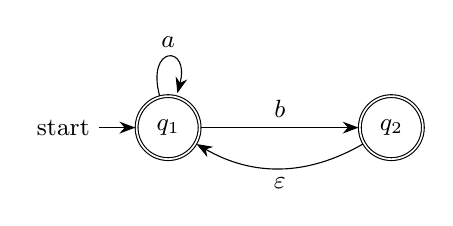
\begin{tikzpicture}[node distance=2cm]
\node[state,initial,accepting] (1) {$q_1$};
\node[state,accepting,right=of 1] (2) {$q_2$};
\path[->] (1) edge[loop above] node {$a$} () edge node {$b$} (2)
          (2) edge[bend left] node {$\eps$} (1);
\end{tikzpicture}\\[-2pt]{\footnotesize the wrong ``shortcut'' NFA: accepts $a$}
\end{minipage}
\end{ans}

\begin{thm}{Fact 2.4. $\emptyset^*=\{\eps\}$.}
\src{Lec05 pp.\,7--13}{2022-23 Q3(c); 2021-22 Q3(a)}
\end{thm}
\begin{proof}
By definition $A^*=\{x_1x_2\cdots x_k\mid k\ge0,\ x_i\in A\}$. For $k=0$ the concatenation of no strings is $\eps$, and $k=0$ needs no
element of $A$, so $\eps\in A^*$ for every $A$. For $k\ge1$ we need $x_1\in A=\emptyset$, impossible. Hence $\emptyset^*=\{\eps\}$.
(In the star NFA: $N_1$ for $\emptyset$ has no accept state, so only the new accepting start state accepts, on input $\eps$.)
\end{proof}

\begin{thm}{Theorem 2.5 (Complement). If $A$ is regular, so is $\overline A=\Sigma^*\setminus A$: swap accepting and non-accepting states of a
\emph{complete DFA}. This fails for NFAs.}
\src{Lec05 pp.\,38--43}{2017-18 Q2(a); 2021-22 Q1(c); 2022-23 Q3(b)}
\end{thm}
\begin{proof}
Let $M=(Q,\Sigma,\delta,q_0,F)$ be a DFA for $A$ with $\delta$ defined for every $(q,a)$ (add a dead state if a move is missing). Let
$M'=(Q,\Sigma,\delta,q_0,Q\setminus F)$. Because $M$ is deterministic and complete, every $w$ has exactly one run, ending in the state
$\dhat(q_0,w)$, and $M'$ has the same run. So
$w\in L(M')\iff \dhat(q_0,w)\in Q\setminus F\iff \dhat(q_0,w)\notin F\iff w\notin A$.
\end{proof}
\textbf{When it does not work.} (i) If the DFA is incomplete, a string on which $M$ ``gets stuck'' is rejected by both $M$ and $M'$
--- complete it with a dead state first. (ii) \textbf{NFAs:} an NFA accepts if \emph{some} branch accepts; after swapping, it accepts if
\emph{some} branch ends in an old non-accepting state. A string can have one branch of each kind and is then accepted by both.

\begin{ans}{NFA counterexample (2021-22 Q1(c), 2022-23 Q3(b))}
\begin{minipage}{0.6\linewidth}
$N$: $q_0\xrightarrow{a}q_0$, $q_0\xrightarrow{a}q_1$, $F=\{q_1\}$; $L(N)=a^+=\{a,aa,\dots\}$, so $\overline{L(N)}=\{\eps\}$ over $\{a\}$.
Swapped NFA has $F'=\{q_0\}$. On $a^n$ one branch stays in $q_0$, so it accepts $\eps,a,aa,\dots$, i.e.\ $a^*\ne\{\eps\}$.
Correct method for NFAs: convert to a DFA (subset construction), complete it, then swap.
\end{minipage}\hfill
\begin{minipage}{0.36\linewidth}\centering
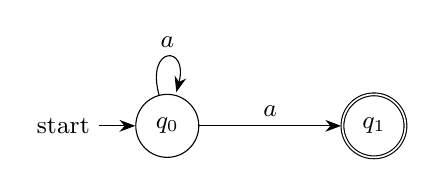
\begin{tikzpicture}[node distance=1.8cm]
\node[state,initial] (0) {$q_0$};
\node[state,accepting,right=of 0] (1) {$q_1$};
\path[->] (0) edge[loop above] node {$a$} () edge node {$a$} (1);
\end{tikzpicture}
\end{minipage}
\end{ans}

\begin{thm}{Theorem 2.6 (Intersection and difference). If $A,B$ are regular, so are $A\cap B$ and $A\setminus B$.}
\src{Lec05 pp.\,44--52}{used in every closure-based non-regularity proof (Section 4.4)}
\end{thm}
\begin{proof}
\emph{Product construction.} DFAs $M_1=(Q_1,\Sigma,\delta_1,q_1,F_1)$, $M_2=(Q_2,\Sigma,\delta_2,q_2,F_2)$. Let $M$ have states $Q_1\times Q_2$,
start $(q_1,q_2)$, $\delta((r,s),a)=(\delta_1(r,a),\delta_2(s,a))$ and $F=F_1\times F_2$. By induction on $|w|$,
$\dhat((q_1,q_2),w)=(\dhat_1(q_1,w),\dhat_2(q_2,w))$ (both machines run side by side), so $M$ accepts iff both accept: $L(M)=A\cap B$.
\emph{De Morgan:} $A\cap B=\overline{\overline A\cup\overline B}$, regular by Theorems 2.1 and 2.5.
\emph{Difference:} $A\setminus B=A\cap\overline B$ (or product with $F=F_1\times(Q_2\setminus F_2)$).
\end{proof}

\begin{thm}{Theorem 2.7 (Reversal). If $A$ is regular, so is $A^R=\{w^R\mid w\in A\}$.}
\src{Lec05 pp.\,53--57}{used in Lec06 p.\,25 ($0^m1^n$, $m<n$)}
\end{thm}
\begin{proof}
From a DFA $M$ for $A$ build an NFA $N$: reverse every arrow, make the old start state the only accept state, add a new start state with
$\eps$-moves to every old accept state. A path $q_0\xrightarrow{w}f$ ($f\in F$) in $M$ is exactly a path $f\xrightarrow{w^R}q_0$ in $N$, so $N$
accepts $w^R$ iff $M$ accepts $w$. (The result is an NFA: after reversal two arrows with the same label may leave one state.)
\end{proof}

% ---------------------------------------------------------------------- 3
\section{Kleene's theorem: regular expressions $=$ finite automata}\markboth{3 Kleene's theorem}{}

\begin{thm}{Theorem 3.1. A language is regular if and only if some regular expression describes it.}
\src{Lec05 pp.\,85--103}{2021-22 Q2(b), 2019-20 Q3(a), 2017-18 Q2(c) use direction ($\Leftarrow$); state elimination uses ($\Rightarrow$)}
\end{thm}
\begin{proof}
($\Leftarrow$, RE $\to$ NFA) Structural induction on $R$.
Base: $R=a$: two states $s\xrightarrow{a}f$; $R=\eps$: one accepting start state; $R=\emptyset$: one non-accepting state.
Step: if $R_1,R_2$ have NFAs, then $R_1\cup R_2$, $R_1R_2$, $R_1^*$ have NFAs by Theorems 2.1--2.3 (Thompson's construction).

($\Rightarrow$, DFA $\to$ RE) Turn the DFA into a GNFA $G$ (arrows labelled by regular expressions): new start $q_s\xrightarrow{\eps}q_0$, new
accept $q_a$ with $f\xrightarrow{\eps}q_a$ for $f\in F$, parallel labels joined by $\cup$, missing arrows labelled $\emptyset$.
$L(G)=L(\text{DFA})$. \textsc{Convert}$(G)$: if $G$ has 2 states return $R(q_s,q_a)$; otherwise remove some $q_{rip}\notin\{q_s,q_a\}$ and
relabel, for all remaining $q_i\ne q_a$, $q_j\ne q_s$,
\[R'(q_i,q_j)=R(q_i,q_j)\ \cup\ R(q_i,q_{rip})\,R(q_{rip},q_{rip})^*\,R(q_{rip},q_j).\]
\emph{Ripping preserves the language.} If $G$ accepts $w$ along $q_s,r_1,\dots,r_m,q_a$, each step not touching $q_{rip}$ is read by the
first term, and each maximal stretch $q_i,q_{rip},\dots,q_{rip},q_j$ is read by the second term; so $G'$ accepts $w$. Conversely each step
$q_i\to q_j$ of $G'$ reads a string of $R(q_i,q_j)$ (a step of $G$) or of $R(q_i,q_{rip})R(q_{rip},q_{rip})^*R(q_{rip},q_j)$ (a path of $G$
through $q_{rip}$); so $G$ accepts $w$. By induction on the number of states, \textsc{Convert}$(G)$ returns an $R$ with
$L(R)=L(G)$.
\end{proof}

% ---------------------------------------------------------------------- 4
\section{Pumping lemma for regular languages}\markboth{4 Regular pumping lemma}{}

\subsection{The lemma, its proof, and why it is shaped as it is}

\begin{thm}{Theorem 4.1 (Pumping lemma). If $A$ is regular, there is a number $p$ (the pumping length) such that every $s\in A$ with
$|s|\ge p$ can be written $s=xyz$ with (1) $xy^iz\in A$ for every $i\ge0$, (2) $|y|>0$, (3) $|xy|\le p$.}
\src{Lec06 pp.\,4--8}{2023-24 Q2(a) (why $|xy|\le p$); 2021-22 Q4(a) (why only for negative proofs)}
\end{thm}
\begin{proof}
Let $M=(Q,\Sigma,\delta,q_1,F)$ be a DFA for $A$ and $p=|Q|$. Let $s=s_1s_2\cdots s_n\in A$, $n\ge p$, and let $r_1,r_2,\dots,r_{n+1}$ be the
states of the run ($r_1=q_1$, $r_{k+1}=\delta(r_k,s_k)$, $r_{n+1}\in F$). The first $p+1$ states $r_1,\dots,r_{p+1}$ are $p+1$ states from a set of
size $p$, so by the pigeonhole principle two are equal: $r_j=r_l$ with $j<l\le p+1$. Put
\[x=s_1\cdots s_{j-1},\qquad y=s_j\cdots s_{l-1},\qquad z=s_l\cdots s_n.\]
$x$ takes $M$ from $r_1$ to $r_j$, $y$ from $r_j$ back to $r_l=r_j$ (a loop), $z$ from $r_l$ to $r_{n+1}\in F$. Going round the loop $i$ times
($i\ge0$) still ends in $r_{n+1}$, so $xy^iz\in A$ --- (1). $j\ne l$ gives $|y|=l-j>0$ --- (2). $l\le p+1$ gives $|xy|=l-1\le p$ --- (3).
\end{proof}
\begin{center}
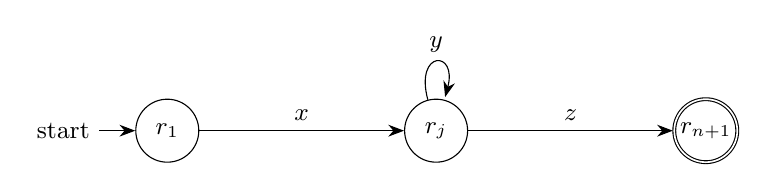
\begin{tikzpicture}[node distance=2.6cm]
\node[state,initial] (a) {$r_1$};
\node[state,right=of a] (b) {$r_j$};
\node[state,accepting,right=of b] (c) {$r_{n+1}$};
\path[->] (a) edge node {$x$} (b) (b) edge[loop above] node {$y$} () (b) edge node {$z$} (c);
\end{tikzpicture}
\end{center}

\textbf{Why $|xy|\le p$ (2023-24 Q2(a)).} \emph{Where it comes from:} the repeated state is found among the first $p+1$ states of the run,
i.e.\ within the first $p$ symbols --- so it is true for free. \emph{Why we need it:} it traps $y$ near the start of $s$, so in a proof we know
what $y$ consists of. Example: $L=\{0^n1^n\}$, $s=0^p1^p$; $|xy|\le p$ forces $y=0^k$, and pumping breaks the count. Without it the adversary
could choose $y$ in the 1s or across the boundary and we would need many cases. \emph{Example automaton:} $L=\{w\in\{0,1\}^*\mid \#_0(w)\equiv0
\pmod 3\}$, DFA $r_0\xrightarrow{0}r_1\xrightarrow{0}r_2\xrightarrow{0}r_0$ with a 1-loop on each state, $p=3$. For $s=10010$ the run is
$r_0\xrightarrow{1}r_0\cdots$: $r_0$ repeats after one symbol, so $x=\eps$, $y=1$, $z=0010$, $|xy|=1\le3$, and $xy^iz=1^i0010\in L$.

\textbf{Why only negative proofs (2021-22 Q4(a)).} The lemma says regular $\Rightarrow$ pumpable. We use the contrapositive (not pumpable
$\Rightarrow$ not regular). The converse is false: $F=\{a^ib^jc^k\mid i,j,k\ge0,\ \text{if } i=1 \text{ then } j=k\}$ is not regular, yet
every string of length $\ge2$ can be pumped (take $y$ = the first symbol, or $y=aa$ when $i=2$). So showing that strings pump proves nothing;
regularity must be shown with a DFA, NFA, regular expression or closure properties.

\begin{trap}\textbf{The 5-step template (Lec06 p.\,11) --- write these exact sentences.}
(1) Assume, for contradiction, that $L$ is regular. (2) Let $p$ be the pumping length. (3) Choose $s\in L$ \emph{in terms of $p$}, check
$s\in L$ and $|s|\ge p$. (4) ``Let $s=xyz$ be \emph{any} split with $|y|>0$, $|xy|\le p$.'' Use $|xy|\le p$ to say what $y$ is.
(5) Choose $i$, show $xy^iz\notin L$. ``This contradicts the pumping lemma, so $L$ is not regular.''\\
\TRAP Never fix $p$ (``let $p=5$''); never choose $x,y,z$ yourself; never show ``$xy^iz\notin L$ for all $i$'' ($i=1$ gives $s$ back).
\end{trap}

\subsection{Direct pumping proofs}
Each proof below follows the template; steps (1), (2) and the closing sentence are the same every time and are written out in 4.2 only.

\begin{thm}{4.2 \ $L=\{0^n1^n\mid n\ge0\}$ is not regular.}
\src{Lec06 pp.\,12--13}{the model answer behind every Skye/BLP question}
\end{thm}
\begin{proof}
Assume, for contradiction, that $L$ is regular, and let $p$ be its pumping length. Choose $s=0^p1^p$; $s\in L$ and $|s|=2p\ge p$. Let $s=xyz$
be any split with $|y|>0$ and $|xy|\le p$. The first $p$ symbols of $s$ are 0s, so $y=0^k$ with $1\le k\le p$. Take $i=0$:
$xz=0^{p-k}1^p$, and $p-k\ne p$, so $xz\notin L$. This contradicts the pumping lemma; hence $L$ is not regular.
\end{proof}

\begin{thm}{4.3 \ Palindromes over $\{a,b\}$ are not regular.}\src{Lec06 pp.\,14--15}{2021-22 Q1(d)(i) (the correct version)}\end{thm}
\begin{proof}
$s=a^pba^p$ (a palindrome, $|s|=2p+1\ge p$). $|xy|\le p$ gives $y=a^k$, $k\ge1$. $i=0$: $xz=a^{p-k}ba^p$ has $p-k$ a's before the $b$ and $p$
after, so it is not a palindrome. Contradiction.
\end{proof}

\begin{thm}{4.4 \ $\{a^nb^nc^n\mid n\ge0\}$ is not regular.}\src{Lec06 pp.\,16--17}{---}\end{thm}
\begin{proof}
$s=a^pb^pc^p$, $|s|=3p$. $y=a^k$, $k\ge1$. $i=2$: $a^{p+k}b^pc^p\notin L$ since $p+k\ne p$. Contradiction.
\end{proof}

\begin{thm}{4.5 \ $\{w\#w\mid w\in\{0,1\}^*\}$ is not regular.}\src{Lec06 pp.\,18--19}{---}\end{thm}
\begin{proof}
$s=0^p1\#0^p1$, $|s|=2p+3$. $y=0^k$, $k\ge1$ (inside the first block). $i=0$: $0^{p-k}1\#0^p1$; the words on the two sides of $\#$ differ.
Contradiction.
\end{proof}

\begin{thm}{4.6 \ $\{a^{n^2}\mid n\ge0\}$ is not regular.}\src{Lec06 pp.\,20--21}{---}\end{thm}
\begin{proof}
$s=a^{p^2}$, $|s|=p^2\ge p$. $y=a^k$, $1\le k\le p$. $i=2$: length $p^2+k$, and $p^2<p^2+k\le p^2+p<p^2+2p+1=(p+1)^2$. It lies strictly between
consecutive squares, so it is not a square. Contradiction.
\end{proof}

\begin{thm}{4.7 \ $L=\{a^{n!}\mid n\ge1\}$ is not regular.}\src{Lec06 p.\,28 (home problem)}{2023-24 Q4(c)}\end{thm}
\begin{proof}
Assume $L$ regular with pumping length $p$. Let $m=\max(p,2)$ and $s=a^{m!}\in L$; $|s|=m!\ge m\ge p$. Any split has $y=a^k$ with
$1\le k\le|xy|\le p\le m$. Take $i=2$: $|xy^2z|=m!+k$, and
\[m!\ <\ m!+k\ \le\ m!+m\ <\ m!+m\cdot m!\ =\ (m+1)!\qquad(\text{since } m!\ge2 \text{ for } m\ge2).\]
So $m!+k$ lies strictly between two consecutive factorials and is not a factorial: $xy^2z\notin L$. Contradiction; $L$ is not regular.
\end{proof}

\begin{thm}{4.8 \ $L=\{a^{2n}b^{3n}a^n\mid n\ge0\}$ is not regular.}\src{Lec06 template}{2019-20 Q4(c)}\end{thm}
\begin{proof}
Assume $L$ regular with pumping length $p$. $s=a^{2p}b^{3p}a^p\in L$ ($n=p$), $|s|=6p\ge p$. Since $|xy|\le p\le2p$, $x$ and $y$ lie in the first
block: $y=a^k$, $k\ge1$. Take $i=2$: $xy^2z=a^{2p+k}b^{3p}a^p$. For it to be in $L$ the $b$-block forces $3n=3p$, i.e.\ $n=p$, so the first
block must be $a^{2p}$; it is $a^{2p+k}\ne a^{2p}$. So $xy^2z\notin L$. Contradiction.
\end{proof}

\begin{thm}{4.9 \ $L=\{a^q\mid q \text{ is prime}\}$ is not regular.}\src{Lec06 pp.\,32--34}{2019-20 Q1(a)}\end{thm}
\begin{proof}
Assume $L$ regular with pumping length $p$. There are infinitely many primes, so choose a prime $q>p$ and $s=a^q\in L$, $|s|=q\ge p$. Any
split has $y=a^k$, $1\le k\le p$. Take $i=q+1$: $|xy^{q+1}z|=q+qk=q(k+1)$. Both $q\ge2$ and $k+1\ge2$, so $q(k+1)$ is composite and
$xy^{q+1}z\notin L$. Contradiction.
\end{proof}

\begin{thm}{4.10 \ $\{a^{2^n}\mid n\ge0\}$ is not regular.}\src{Lec06 p.\,27}{---}\end{thm}
\begin{proof}
Choose $m$ with $2^m>p$ and $s=a^{2^m}$. $y=a^k$, $1\le k\le p<2^m$. $i=2$: $2^m<2^m+k<2^m+2^m=2^{m+1}$ --- not a power of two. Contradiction.
\end{proof}

\begin{thm}{4.11 \ $\{a^{F_n}\mid n\ge0\}$ ($F_n$ Fibonacci) is not regular.}\src{Lec06 pp.\,38--40}{---}\end{thm}
\begin{proof}
Choose $m\ge3$ with $F_{m-1}>p$; $s=a^{F_m}$, $|s|=F_m>p$. $y=a^k$, $1\le k\le p<F_{m-1}$. $i=2$: $F_m<F_m+k<F_m+F_{m-1}=F_{m+1}$,
strictly between consecutive Fibonacci numbers. Contradiction. (\TRAP $F_m>p$ is not enough; we need $k\le p<F_{m-1}$.)
\end{proof}

\begin{thm}{4.12 \ $\{ww\mid w\in\{0,1\}^*\}$ is not regular.}\src{Lec06 template}{2017-18 Q3(b)(i), 2020 Q1(b)(i) (the correct proof)}\end{thm}
\begin{proof}
$s=0^p1\,0^p1\in L$, $|s|=2p+2$. $y=0^k$, $k\ge1$, inside the first block. $i=0$: $t=0^{p-k}1\,0^p1$. If $t=uu$, then $u$ ends with the last
symbol of $t$, a 1, and each half contains exactly one of the two 1s; so $u=0^{p-k}1$ (first half) and $u=0^p1$ (second half), forcing
$k=0$. Contradiction. (\TRAP $s=0^p0^p$ does not work: it pumps fine with $y=00$.)
\end{proof}

\begin{thm}{4.13 \ $\{w\mid n_0(w)=2n_1(w)\}$ and $\{w\mid n_0(w)=3n_1(w)\}$ are not regular.}
\src{Lec06 template}{2017-18 Q3(b)(ii), 2020 Q1(b)(ii)}\end{thm}
\begin{proof}
For $c\in\{2,3\}$: $s=0^{cp}1^p\in L$, $|s|=(c+1)p\ge p$. The first $p$ symbols are 0s, so $y=0^k$, $k\ge1$. $i=2$: $0^{cp+k}1^p$ has
$n_0=cp+k\ne cp=c\,n_1$. Contradiction.
\end{proof}

\begin{thm}{4.14 \ $\{0^n1^n0^n\mid n\ge0\}$ is not regular.}\src{Lec06 template}{2017-18 Q3(b)(iii) (the correct proof)}\end{thm}
\begin{proof}
$s=0^p1^p0^p$, $|s|=3p\ge p$. $y=0^k$, $k\ge1$. $i=0$: $0^{p-k}1^p0^p\notin L$ (first block $\ne$ middle block). Contradiction.
\end{proof}

\subsection{Non-regularity by closure properties}
Pattern: assume $L$ regular; combine it with regular languages using operations that preserve regularity; reach a language already known
to be non-regular (usually $\{0^n1^n\}$). That contradiction proves $L$ is not regular.

\begin{thm}{4.15 \ $L_{\ne}=\{0^m1^n\mid m\ne n\}$ is not regular.}\src{Lec06 p.\,24}{---}\end{thm}
\begin{proof}
If $L_{\ne}$ were regular, then $0^*1^*\setminus L_{\ne}=\{0^n1^n\}$ would be regular (closure under difference). It is not (4.2).
\end{proof}

\begin{thm}{4.16 \ $L_<=\{0^m1^n\mid m<n\}$ is not regular.}\src{Lec06 p.\,25}{---}\end{thm}
\begin{proof}
If $L_<$ were regular, reversing and swapping $0\leftrightarrow1$ (both preserve regularity: Theorem 2.7 and a relabelled DFA) gives
$L_>=\{0^m1^n\mid m>n\}$ regular, so $L_<\cup L_>=L_{\ne}$ would be regular --- contradicting 4.15.
\end{proof}

\begin{thm}{4.17 \ $\{w\in\{0,1\}^*\mid \#_0(w)\ne\#_1(w)\}$ is not regular.}\src{Lec06 pp.\,29--31}{---}\end{thm}
\begin{proof}
If it were regular, its complement $E=\{w\mid\#_0(w)=\#_1(w)\}$ would be regular, and then $E\cap0^*1^*=\{0^n1^n\}$ would be regular. It is
not. (\TRAP the complement is $E$, not $\{0^n1^n\}$; the intersection with $0^*1^*$ is needed.)
\end{proof}

\begin{thm}{4.18 \ $L_{comp}=\{a^t\mid t \text{ composite}\}$ is not regular.}\src{Lec06 pp.\,35--37}{---}\end{thm}
\begin{proof}
$a^*=L_{prime}\cup L_{comp}\cup\{\eps,a\}$ (0 and 1 are neither prime nor composite). If $L_{comp}$ were regular, then
$a^*\setminus(L_{comp}\cup\{\eps,a\})=L_{prime}$ would be regular, contradicting 4.9.
\end{proof}

\begin{thm}{4.19 \ Over $\Sigma=\{a,b,c\}$, $\{w\mid\#_{ab}(w)=\#_{ba}(w)\}$ is not regular.}\src{Lec06 pp.\,41--48}{---}\end{thm}
\begin{proof}
Let $R=(abc)^*(bac)^*$ (regular). For $w=(abc)^m(bac)^n$, $\#_{ab}=m$ and $\#_{ba}=n$, so $L\cap R=K=\{(abc)^n(bac)^n\}$. If $L$ were regular,
so would be $K$. Pump $K$: $s=(abc)^p(bac)^p$, $|s|=6p$; $|xy|\le p<3p$ puts $y$ inside $(abc)^p$; let $k=|y|$, take $i=0$. If $3\nmid k$:
$|xz|=6p-k$ is not a multiple of 3 (hence not 6), but every string of $K$ has length $6n$. If $k=3r$: deleting $3r$ consecutive symbols from
a period-3 word leaves $(abc)^{p-r}$, so $xz=(abc)^{p-r}(bac)^p\notin K$. Either way, contradiction. (Over $\{a,b\}$ the language
\emph{is} regular: $\#_{ab}-\#_{ba}$ depends only on the first and last symbols.)
\end{proof}

\subsection{``What is wrong with this argument?'' questions}

\begin{ans}{4.20 \ Minimum pumping length --- 2022-23 Q2(b): $L=\{a^{2+3k}\}\cup\{b^{10+12k}\}$, $k\ge0$. Are 3, 5, 9, 24 pumping lengths?}
$L=\{a^2,a^5,a^8,\dots\}\cup\{b^{10},b^{22},b^{34},\dots\}$. $p$ is a pumping length if \emph{every} $s\in L$ with $|s|\ge p$ has a good split.\\
\emph{a-strings.} $y=a^j$; pumping up keeps the length $\equiv2\pmod3$ only if $3\mid j$; pumping down needs $2+3k-j\ge2$. So $a^2$ cannot be
pumped, and $a^{2+3k}$ ($k\ge1$) pumps with $x=\eps$, $y=a^3$ (needs $p\ge3$).\\
\emph{b-strings.} $y=b^j$ needs $12\mid j$, and pumping down needs $k\ge1$. So $b^{10}$ can never be pumped ($\Rightarrow p>10$), and any
$b$-string's $y$ has length $\ge12$ with $|xy|\le p$ ($\Rightarrow p\ge12$). For $p\ge12$ every $b^{10+12k}$ with $10+12k\ge p$ has $k\ge1$ and
pumps with $x=\eps$, $y=b^{12}$: $xy^iz=b^{10+12(k-1+i)}\in L$.\\
\textbf{Answer.} 3, 5, 9: \textbf{not} pumping lengths --- witness $b^{10}$ (length $\ge p$, unpumpable). 24: \textbf{is} one (a-strings: $y=a^3$;
b-strings of length $\ge24$ are $b^{34},b^{46},\dots$: $y=b^{12}$). Minimum: $p=11$ fails on $b^{22}$ (its $y$ would need length 12), $p=12$
works. \textbf{Minimum pumping length $=12$.}
\end{ans}

\begin{ans}{4.21 \ Skye --- 2017-18 Q3(b) and 2020 Q1(b)}
\textbf{(i) $L_1=\{ww\}$: ``choose $0^p0^p$, $x=\eps$, $y=(00)^k$; all $xy^iz\in L_1$, so $L_1$ is regular.''} Wrong twice. The lemma is
only a \emph{necessary} condition: showing strings pump never proves regularity (Theorem 4.1, negative proofs only). And the prover may not
choose $y$. $L_1$ is in fact not regular (4.12, with $s=0^p10^p1$).\\[2pt]
\textbf{(ii) $L_2=\{n_0=2n_1\}$ with $0^{2p}1^p$, $y=01$ (2017-18); $\{n_0=3n_1\}$ with $0^{3p}1^p$, $y=0001$ (2020): ``we failed to
contradict the lemma''.} The chosen $y$ is illegal: $|xy|\le p$ forces $y$ inside the leading 0s, so $y=0^k$; and we must handle every
legal $y$, not pick one. With the legal $y=0^k$, pumping up breaks the count (4.13): the language is not regular.\\[2pt]
\textbf{(iii) $L_3=\{0^n1^n0^n\}$ with $0^k1^k0^k$, $k=\lfloor p/3\rfloor$: ``$xy^iz\notin L_3$ for every $i$ and all $y$''.} Two errors.
$|s|=3\lfloor p/3\rfloor$ may be $<p$, and the lemma says nothing about such strings. And ``for every $i$'' is false: $i=1$ gives $s\in L_3$; one
$i$ suffices. Correct proof: 4.14 with $s=0^p1^p0^p$.
\end{ans}

\begin{ans}{4.22 \ B.\,L.\,Perfunctory --- 2021-22 Q1(d)}
\textbf{(i) Palindromes with $w=00011000$.} Not acceptable: $w$ is a fixed string and does not depend on $p$; if $p>8$ the lemma says nothing
about it, and $w$ does not start with $0^p$. The conclusion is true; the correct proof uses $s=0^p10^p$ (4.3).\\[2pt]
\textbf{(ii) Equal 0s and 1s with $w=0^{p/4}1^{p/4}0^{p/4}1^{p/4}$.} Not acceptable: $|w|=p$, so $|xy|\le p$ allows $y$ anywhere in $w$, not only
in the first 0s. The adversary picks $y=01$, which keeps the counts equal for every $i$. Correct: $s=0^p1^p$, $y=0^k$, $i=2$.\\[2pt]
\textbf{(iii) $\{0^{2n}\}$ with $w=0^{2p}$, $x=\eps$, $y=0$.} Not acceptable: the prover may not choose the split. The adversary picks $y=00$ (legal for
$p\ge2$) and $xy^iz=0^{2p-2+2i}\in L$ for all $i$. In fact $\{0^{2n}\}=(00)^*$ is regular, so no valid proof exists.
\end{ans}

\begin{ans}{4.23 \ Primes --- 2019-20 Q1(a): is the start ``Given $p$, let $w=a^p$'' acceptable?}
No. $p$ is whatever the lemma supplies and need not be prime (e.g.\ $p=4$); then $a^p\notin L$ and the lemma says nothing about it. The string
must be in $L$. Correct start: choose a prime $q>p$ and $s=a^q$, then pump with $i=q+1$ (4.9).
\end{ans}

% ---------------------------------------------------------------------- 5
\section{Context-free grammars: correctness and ambiguity}\markboth{5 CFG proofs}{}

\begin{thm}{Theorem 5.1. Every regular language is context-free.}\src{Lec07 pp.\,48--50}{---}\end{thm}
\begin{proof}
Let DFA $M=(Q,\Sigma,\delta,q_0,F)$ recognise $L$. Make a variable $R_q$ for each state, start variable $R_{q_0}$, a rule $R_q\to aR_r$ for each
$\delta(q,a)=r$, and $R_q\to\eps$ for each $q\in F$. By induction on $|w|$: $R_{q_0}\Rightarrow^*wR_q$ iff $\dhat(q_0,w)=q$ (each step
of the derivation is one move of $M$). A derivation ends with $R_q\to\eps$ only for $q\in F$, so $R_{q_0}\Rightarrow^*w$ iff
$\dhat(q_0,w)\in F$. Hence $L(G)=L(M)=L$.
\end{proof}

\begin{thm}{Theorem 5.2. $G:\ S\to0S1S\mid1S0S\mid\eps$ generates exactly $\{w\in\{0,1\}^*\mid \#_0(w)=\#_1(w)\}$.}
\src{Lec07 pp.\,35--37}{grammar asked in 2019-20 Q5, 2020 Q5, 2017-18 Q5 --- prove it to get full marks}\end{thm}
\begin{proof}
\emph{Soundness ($L(G)\subseteq E$).} Induction on derivation length: every sentential form has equally many 0s and 1s, because each rule
adds either nothing or exactly one 0 and one 1.

\emph{Completeness ($E\subseteq L(G)$).} Strong induction on $|w|$. $w=\eps$: $S\to\eps$. Let $w\ne\eps$ be balanced and start with 0 (the
case 1 is symmetric with $S\to1S0S$). Let $d(u)=\#_0(u)-\#_1(u)$ for prefixes $u$. $d=1$ after the first symbol and $d=0$ at the end, and
$d$ changes by $\pm1$ per symbol, so there is a first prefix after the first symbol with $d=0$; the symbol that brought $d$ from 1 to 0 is a 1.
So $w=0x1y$ where $d(0x)=1$ (so $x$ is balanced) and $d(0x1)=0$ (so $y$ is balanced). $|x|,|y|<|w|$, so by the hypothesis
$S\Rightarrow^*x$ and $S\Rightarrow^*y$; hence $S\Rightarrow0S1S\Rightarrow^*0x1y=w$.
\end{proof}

\begin{thm}{Definitions (for every ambiguity question).}\src{Lec07 pp.\,54, 62}{2021-22 Q6, 2019-20 Q6, 2021-22 Q4(d)}\end{thm}
A string $w$ is \textbf{derived ambiguously} in $G$ if it has two different parse trees (equivalently two different \emph{leftmost}
derivations). $G$ is \textbf{ambiguous} if some string is derived ambiguously. A CFL is \textbf{inherently ambiguous} if \emph{every} CFG for
it is ambiguous. Ambiguity is a property of the grammar; inherent ambiguity is a property of the language. To \emph{prove} a grammar
ambiguous, exhibit one string and two leftmost derivations (or two parse trees). Two different derivations that give the same tree (e.g.\ a
leftmost and a rightmost one) prove nothing.

\begin{thm}{5.3 \ $E\to E+E\mid E\times E\mid(E)\mid a$ is ambiguous; an unambiguous grammar for the same language.}
\src{Lec07 pp.\,55--58}{2017-18 Q6}\end{thm}
\begin{proof}
$a+a\times a$ has two leftmost derivations:
\[E\Rightarrow E+E\Rightarrow a+E\Rightarrow a+E\times E\Rightarrow a+a\times E\Rightarrow a+a\times a\quad(\text{tree } a+(a\times a)),\]
\[E\Rightarrow E\times E\Rightarrow E+E\times E\Rightarrow a+E\times E\Rightarrow a+a\times E\Rightarrow a+a\times a\quad(\text{tree } (a+a)\times a).\]
Different first steps give different roots ($+$ vs $\times$), so the trees differ and $G$ is ambiguous.
\emph{Removing the ambiguity:} add precedence levels and left associativity,
\[E\to E+T\mid T,\qquad T\to T\times F\mid F,\qquad F\to(E)\mid a.\]
It generates the same expressions. A parse is unique: $E\to E+T$ must split at the \emph{last} $+$ outside parentheses, $T\to T\times F$ at the
last $\times$ outside parentheses, and $F$ is either $a$ or a parenthesised $E$. So $a+a\times a$ has only the tree $a+(a\times a)$.
\end{proof}

\begin{thm}{5.4 \ $S\to AB\mid C,\ A\to aAb\mid ab,\ B\to cB\mid c,\ C\to aCc\mid aDc,\ D\to bD\mid b$ is ambiguous.}
\src{Lec07 pp.\,54, 62--63}{2021-22 Q6; 2019-20 Q6 (also 2023-24 Q5: this is a grammar for $\{a^ib^jc^k\mid i=j \text{ or } i=k;\ i,j,k\ge1\}$)}\end{thm}
\begin{proof}
$A$ generates $a^nb^n$ and $B$ generates $c^m$ ($n,m\ge1$), so $AB$ gives $\{a^nb^nc^m\}$ ($i=j$). $C$ generates $a^nb^jc^n$ ($i=k$). The string
$abc$ (and every $a^nb^nc^n$) satisfies both:
\[S\Rightarrow AB\Rightarrow abB\Rightarrow abc,\qquad S\Rightarrow C\Rightarrow aDc\Rightarrow abc.\]
Two leftmost derivations (different first step), so two parse trees: the grammar is ambiguous.
\end{proof}
\textbf{Is the language inherently ambiguous?} Yes --- it is the standard kind of example: the strings $a^nb^nc^n$ belong to both ``halves'',
and any grammar must generate them once through the $i=j$ mechanism and once through the $i=k$ mechanism. The full proof needs Ogden's
lemma, which is not in the syllabus; in the exam give the definitions, this example and that reason. The slides' example (Lec07 p.\,62) is
the same idea:

\begin{thm}{5.5 \ $L=\{a^nb^nc^md^m\}\cup\{a^nb^mc^md^n\}$ ($n,m\ge1$): a grammar, and its ambiguity.}
\src{Lec07 pp.\,62--63}{2022-23 Q6; 2020 Q6}\end{thm}
\begin{proof}
$S\to AB\mid C,\ A\to aAb\mid ab,\ B\to cBd\mid cd,\ C\to aCd\mid aDd,\ D\to bDc\mid bc.$
$AB$ matches $a$ with $b$ and $c$ with $d$; $C$ matches the outer $a,d$ and the inner $b,c$. The string $abcd$ is in both parts:
\[S\Rightarrow AB\Rightarrow abB\Rightarrow abcd,\qquad S\Rightarrow C\Rightarrow aDd\Rightarrow abcd,\]
two leftmost derivations, so the grammar is ambiguous. $L$ is inherently ambiguous (every grammar generates $a^nb^nc^nd^n$ in two ways), which
is why no repair is possible here, unlike 5.3.
\end{proof}

\begin{thm}{5.6 \ Why ``context-free''?}\src{Lec07 p.\,14}{2023-24 Q3(c); 2021-22 Q1(e)}\end{thm}
Every rule has the form $A\to\gamma$ with a single variable on the left. A variable may be replaced by $\gamma$ wherever it appears,
whatever surrounds it (its \emph{context}). In a context-sensitive rule such as $aAb\to a\gamma b$, $A$ may be rewritten only when it sits
between $a$ and $b$. Example: in $S\to0S1\mid\eps$ the $S$ in $00S11$ is replaced the same way as in $0S1$.

% ======================================================================= PART B
\clearpage
\section*{Part B --- Atif Sir}\addcontentsline{toc}{section}{Part B --- Atif Sir}

\section{Chomsky normal form}\markboth{6 CNF}{}

\begin{thm}{Theorem 6.1. Every CFL $L$ with $\eps\notin L$ has a grammar in CNF (all rules $A\to BC$ or $A\to a$).}
\src{Lecture 2 pp.\,19--35}{the conversions in 2021-22 Q5 and 2017-18 Q7(a) follow these steps}\end{thm}
\begin{proof}
Start from any CFG $G$ for $L$ and apply, in this order, steps that each keep the language (minus $\eps$):
\begin{enumerate}
\item \emph{Remove $\eps$-rules.} Find the nullable variables ($A\Rightarrow^*\eps$). For each rule, add every version with some nullable
occurrences deleted (but never an empty body); then drop all $A\to\eps$. Any derivation of a non-empty $w$ that used $\eps$-rules is
matched by one that deletes those variables at the start, so nothing but $\eps$ is lost.
\item \emph{Remove unit rules $A\to B$.} Find all unit pairs $(A,B)$ ($A\Rightarrow^*B$ by unit rules); for each, give $A$ every non-unit body of
$B$; drop unit rules. A chain of unit steps followed by a non-unit step is replaced by one step.
\item \emph{Remove useless symbols.} First delete non-generating symbols (cannot derive a terminal string), then unreachable ones (not
reachable from $S$). They occur in no derivation of a terminal string, so the language is unchanged. (Order matters: generating first.)
\item \emph{Put bodies in CNF.} In every body of length $\ge2$ replace each terminal $a$ by a new $X_a$ with $X_a\to a$. Break
$A\to B_1B_2\cdots B_k$ ($k\ge3$) into $A\to B_1C_1,\ C_1\to B_2C_2,\dots,C_{k-2}\to B_{k-1}B_k$ with new $C_i$. Each new variable has one
rule, so derivations correspond one to one.
\end{enumerate}
After step 2 every body of length 1 is a terminal; after step 4 every longer body is two variables: the grammar is in CNF.
\end{proof}

% ---------------------------------------------------------------------- 7
\section{Pushdown automata}\markboth{7 PDA proofs}{}

Notation (HMU): $P=(Q,\Sigma,\Gamma,\delta,q_0,Z_0,F)$; ID $(q,w,\gamma)$;
$L(P)=\{w\mid(q_0,w,Z_0)\vdash^*(q,\eps,\alpha),\ q\in F\}$ (final state), $N(P)=\{w\mid(q_0,w,Z_0)\vdash^*(q,\eps,\eps)\}$ (empty stack).

\begin{thm}{Theorem 7.1. A language is $N(P_N)$ for some PDA $P_N$ iff it is $L(P_F)$ for some PDA $P_F$
(acceptance by empty stack and by final state are equivalent).}
\src{Lecture 3 pp.\,102--109}{2019-20 Q10(a)}\end{thm}
\begin{proof}
\textbf{(Empty stack $\Rightarrow$ final state.)} Given $P_N=(Q,\Sigma,\Gamma,\delta_N,q_0,Z_0)$, use a new bottom marker $X_0\notin\Gamma$, a new start
state $p_0$ and a new accepting state $p_f$:
$P_F=(Q\cup\{p_0,p_f\},\Sigma,\Gamma\cup\{X_0\},\delta_F,p_0,X_0,\{p_f\})$ with
\begin{enumerate}
\item $\delta_F(p_0,\eps,X_0)=\{(q_0,Z_0X_0)\}$ (push $P_N$'s start symbol above the marker and start $P_N$);
\item $\delta_F(q,a,Y)=\delta_N(q,a,Y)$ for all $q\in Q$, $a\in\Sigma\cup\{\eps\}$, $Y\in\Gamma$ (run $P_N$);
\item $\delta_F(q,\eps,X_0)\ni(p_f,\eps)$ for every $q\in Q$ (marker exposed $\Rightarrow$ $P_N$ has emptied its stack: accept).
\end{enumerate}
If $(q_0,w,Z_0)\vdash^*_N(q,\eps,\eps)$ then $(p_0,w,X_0)\vdash(q_0,w,Z_0X_0)\vdash^*(q,\eps,X_0)\vdash(p_f,\eps,\eps)$ (the same moves, with
$X_0$ untouched underneath). Conversely $P_F$ enters $p_f$ only by rule 3, i.e.\ only when $X_0$ is on top, which happens exactly when the
simulated $P_N$ has an empty stack after reading the same input. So $L(P_F)=N(P_N)$.

\textbf{(Final state $\Rightarrow$ empty stack.)} Given $P_F=(Q,\Sigma,\Gamma,\delta_F,q_0,Z_0,F)$, let\\
$P_N=(Q\cup\{p_0,p\},\Sigma,\Gamma\cup\{X_0\},\delta_N,p_0,X_0)$ with
\begin{enumerate}
\item $\delta_N(p_0,\eps,X_0)=\{(q_0,Z_0X_0)\}$;
\item $\delta_N(q,a,Y)\supseteq\delta_F(q,a,Y)$ for $q\in Q$, $a\in\Sigma\cup\{\eps\}$, $Y\in\Gamma$ (run $P_F$);
\item $\delta_N(q,\eps,Y)\ni(p,\eps)$ for $q\in F$, $Y\in\Gamma\cup\{X_0\}$ (in an accepting state, may start emptying);
\item $\delta_N(p,\eps,Y)=\{(p,\eps)\}$ for $Y\in\Gamma\cup\{X_0\}$ (pop everything).
\end{enumerate}
If $P_F$ accepts $w$ in $q\in F$ with stack $\alpha$, then $P_N$ follows the same moves to $(q,\eps,\alpha X_0)$, goes to $p$ and pops $\alpha X_0$.
Conversely $P_N$'s stack can become empty only after $X_0$ is popped, which only state $p$ does, and $p$ is entered only from a state of $F$;
so $P_F$ was in an accepting state after reading all of $w$. The marker $X_0$ stops $P_N$ from accepting when $P_F$ happens to empty its own
stack in a non-accepting state. So $N(P_N)=L(P_F)$.
\end{proof}

\begin{thm}{Theorem 7.2. For every CFG $G$ there is a PDA $P$ with $N(P)=L(G)$.}\src{Lecture 3 pp.\,110--115 (proof skipped in slides)}{---}\end{thm}
\begin{proof}
For $G=(V,T,R,S)$ let $P=(\{q\},T,V\cup T,\delta,q,S)$ with $\delta(q,\eps,A)=\{(q,\beta)\mid A\to\beta\in R\}$ (expand the top variable,
guessing the rule) and $\delta(q,a,a)=\{(q,\eps)\}$ (match a terminal). \emph{Invariant:} if $P$ has read $x$ and its stack is $\alpha$, then
$S\Rightarrow^*_{lm}x\alpha$; and conversely every leftmost sentential form $xA\alpha$ is reached with $x$ read and $A\alpha$ on the stack
(induction on the number of moves / derivation steps). With $\alpha=\eps$: $P$ empties its stack after reading $w$ iff $S\Rightarrow^*_{lm}w$.
\end{proof}
\emph{The converse} (PDA $\to$ CFG, variables $[pXq]$ = ``starting in $p$, $X$ is eventually popped, ending in $q$''; rules
$S\to[q_0Z_0p]$ and $[qXr_k]\to a[rY_1r_1][r_1Y_2r_2]\cdots[r_{k-1}Y_kr_k]$ for each $(r,Y_1\cdots Y_k)\in\delta(q,a,X)$) is stated in the slides
with the proof skipped (pp.\,116--122). Together: CFG $=$ PDA by empty stack $=$ PDA by final state.

% ---------------------------------------------------------------------- 8
\section{Pumping lemma for context-free languages}\markboth{8 CFL pumping lemma}{}

\begin{thm}{Lemma 8.1 (Size of parse trees). In a parse tree of a CNF grammar whose yield is a terminal string $w$, if the longest path
(counted in edges) has length $n$, then $|w|\le2^{n-1}$.}\src{Lecture 3 p.\,126 (proof skipped)}{given in 2022-23 Q9, but quick to prove}\end{thm}
\begin{proof}
Induction on $n$. $n=1$: the tree is a root $A$ with one leaf $a$ ($A\to a$), so $|w|=1=2^0$. $n>1$: the root uses $A\to BC$; the subtrees
of $B$ and $C$ have longest paths $\le n-1$, so by the hypothesis their yields have length $\le2^{n-2}$ each, and
$|w|\le2\cdot2^{n-2}=2^{n-1}$.
\end{proof}

\begin{thm}{Theorem 8.2 (Pumping lemma for CFLs). If $L$ is a CFL, there is a constant $n$ such that every $z\in L$ with $|z|\ge n$ can be
written $z=uvwxy$ with (1) $|vwx|\le n$, (2) $vx\ne\eps$, (3) $uv^iwx^iy\in L$ for all $i\ge0$.}
\src{Lecture 3 pp.\,123--129; Hakim Lec07 pp.\,66--68 (Sipser form $w=uvxyz$, $|vxy|\le p$, $|vy|>0$)}{2022-23 Q9 (state and prove)}\end{thm}
\begin{proof}
If $L=\emptyset$ or $L=\{\eps\}$ there is nothing to prove; otherwise take a CNF grammar $G=(V,T,P,S)$ for $L\setminus\{\eps\}$ (Theorem
6.1) and let $m=|V|$. Choose $n=2^m$.

\emph{A long path exists.} Let $z\in L$, $|z|\ge n=2^m$. If every path of a parse tree for $z$ had length $\le m$, Lemma 8.1 would give
$|z|\le2^{m-1}<2^m$. So the longest path has length $k+1$ with $k\ge m$; it contains $k+1$ variables $A_0=S,A_1,\dots,A_k$ and then a terminal.

\emph{A variable repeats.} Look at the last $m+1$ variables $A_{k-m},\dots,A_k$. There are only $m$ different variables, so by the pigeonhole
principle $A_i=A_j=A$ for some $k-m\le i<j\le k$.

\emph{The split.} Let $T_i$ and $T_j$ be the subtrees rooted at $A_i$ and $A_j$ ($T_j$ inside $T_i$). Let $w$ be the yield of $T_j$; the yield
of $T_i$ is then $vwx$, and $z=uvwxy$ (figure).
\begin{itemize}
\item \emph{(2) $vx\ne\eps$.} $A_i$ is not a leaf parent (it has the variable $A_j$ below it), so it uses a rule $A_i\to BC$. $T_j$ lies inside
one of the two subtrees, say $B$'s; then the whole yield of $C$ (non-empty: CNF has no $\eps$-rules) is part of $x$. So $vx\ne\eps$.
\item \emph{(1) $|vwx|\le n$.} The path from $A_i$ down to the leaf on our longest path has length $k-i+1\le m+1$. Every path in $T_i$ has length
$\le m+1$ (a longer one, joined to the path $S\to A_i$, would be longer than the longest path). By Lemma 8.1, $|vwx|\le2^{m}=n$.
\item \emph{(3) Pumping.} Because $A_i=A_j$: replacing $T_i$ by $T_j$ gives a valid tree with yield $uwy=uv^0wx^0y$ (figure b). Replacing
$T_j$ by a copy of $T_i$ gives yield $uv^2wx^2y$ (figure c); repeating gives $uv^iwx^iy$ for every $i\ge2$. All are in $L$.
\end{itemize}
\vspace{-6pt}
\end{proof}
\begin{center}
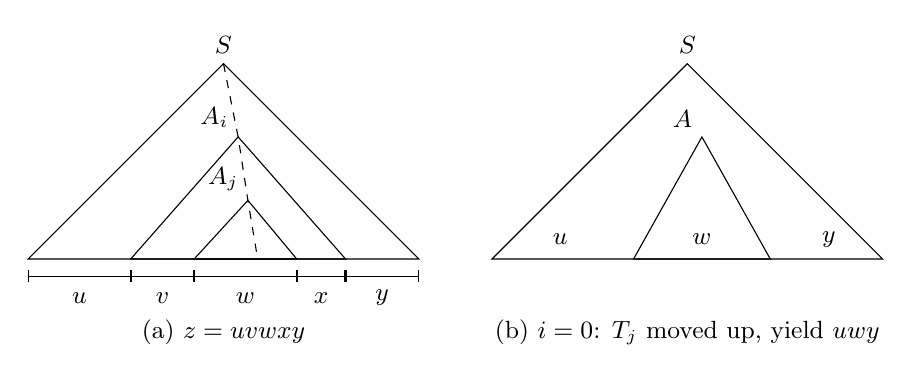
\begin{tikzpicture}[scale=0.62,every node/.style={font=\small}]
\draw (0,0) node[above]{$S$} -- (-4,-4) -- (4,-4) -- cycle;
\draw (0.3,-1.5) node[above left]{$A_i$} -- (-1.9,-4) -- (2.5,-4) -- cycle;
\draw (0.5,-2.8) node[above left]{$A_j$} -- (-0.6,-4) -- (1.5,-4) -- cycle;
\draw[dashed] (0,0)--(0.3,-1.5)--(0.5,-2.8)--(0.7,-4);
\foreach \a/\b/\l in {-4/-1.9/u,-1.9/-0.6/v,-0.6/1.5/w,1.5/2.5/x,2.5/4/y}
  {\draw[|-|] (\a,-4.35)--(\b,-4.35); \node at ({(\a+\b)/2},-4.8) {$\l$};}
\node at (0,-5.5) {(a) $z=uvwxy$};
\begin{scope}[xshift=9.5cm]
\draw (0,0) node[above]{$S$} -- (-4,-4) -- (4,-4) -- cycle;
\draw (0.3,-1.5) node[above left]{$A$} -- (-1.1,-4) -- (1.7,-4) -- cycle;
\node at (0.3,-3.6) {$w$};\node at (-2.6,-3.6){$u$};\node at (2.9,-3.6){$y$};
\node at (0,-5.5) {(b) $i=0$: $T_j$ moved up, yield $uwy$};
\end{scope}
\end{tikzpicture}\\
{\footnotesize (c) for $i=2$, put a copy of $T_i$ where $T_j$ was: yield $uv\,vwx\,xy=uv^2wx^2y$.}
\end{center}

\begin{trap}\textbf{Template for a non-CFL proof (2023-24 Q7, 2021-22 Q8: ``give a non-CFL and prove it'').} (1) Assume $L$ is a CFL; let $n$ be
the constant. (2) Choose $z\in L$ using $n$, $|z|\ge n$. (3) ``Let $z=uvwxy$ be \emph{any} split with $|vwx|\le n$, $vx\ne\eps$.'' Use
$|vwx|\le n$ to say which blocks $vwx$ can touch. (4) Cover \emph{every} case, pick $i$ (usually 0 or 2), show $uv^iwx^iy\notin L$.
(5) Contradiction, so $L$ is not context-free.
\TRAP You choose $z$ and $i$, never $u,v,w,x,y$. Pump $v$ and $x$ \emph{together}. Remember $v$ or $x$ alone may be empty.\end{trap}

\begin{thm}{8.3 \ $L=\{0^m1^m2^m\mid m\ge1\}$ is not context-free. (Best answer for ``give a non-CFL and prove it''.)}
\src{Lecture 3 pp.\,123--125; Lec07 pp.\,73--77}{2023-24 Q7; 2021-22 Q8}\end{thm}
\begin{proof}
Assume $L$ is a CFL and let $n$ be its constant. Choose $z=0^n1^n2^n\in L$, $|z|=3n\ge n$. Let $z=uvwxy$ be any split with $|vwx|\le n$ and
$vx\ne\eps$. Since $|vwx|\le n$, $vwx$ cannot contain both a 0 and a 2 (between them lie all $n$ 1s, so that would need length $\ge n+2$).
\begin{itemize}
\item \emph{$v$ or $x$ contains two different symbols.} Then $uv^2wx^2y$ has symbols out of order (e.g.\ a 1 before a 0), so it is not
in $0^*1^*2^*$, hence not in $L$.
\item \emph{$v$ and $x$ each consist of one symbol.} \emph{Case: $vwx$ has no 2.} Then $uwy$ ($i=0$) still has $n$ 2s but fewer 0s or fewer
1s (since $vx\ne\eps$ removes at least one 0 or 1). \emph{Case: $vwx$ has no 0.} Then $uwy$ has $n$ 0s but fewer 1s or 2s.
\end{itemize}
In every case some $uv^iwx^iy\notin L$, contradicting the lemma. So $L$ is not context-free.
\end{proof}

\begin{thm}{8.4 \ $L=\{0^i1^j2^i3^j\mid i,j\ge1\}$ (equivalently $\{a^nb^mc^nd^m\}$) is not context-free.}
\src{Lecture 3 p.\,123; Lec07 pp.\,78--80}{alternative answer for 2023-24 Q7, 2021-22 Q8}\end{thm}
\begin{proof}
$z=0^n1^n2^n3^n$, $|z|=4n$. $|vwx|\le n$ means $vwx$ touches at most two \emph{adjacent} blocks. If $v$ or $x$ mixes two symbols, $uv^2wx^2y$ is
out of order. Otherwise pumping ($i=0$) changes the length of one or two adjacent blocks and leaves their partners unchanged: if it changes
the 0-block, the 2-block (not adjacent) is untouched, so $\#0\ne\#2$; if it changes only the 1- and/or 2-block, then either $\#1\ne\#3$ or
$\#2\ne\#0$; similarly for the 3-block. Since $vx\ne\eps$, at least one block changes. Contradiction.
\end{proof}

\begin{thm}{8.5 \ $L=\{ww\mid w\in\{0,1\}^*\}$ is not context-free.}\src{Lecture 3 p.\,123}{alternative answer for 2023-24 Q7, 2021-22 Q8}\end{thm}
\begin{proof}
Assume $L$ is a CFL with constant $n$. Choose $z=0^n1^n0^n1^n\in L$, $|z|=4n\ge n$. Let $z=uvwxy$ be any split with $|vwx|\le n$, $vx\ne\eps$,
and take $i=0$: $t=uwy$. If $|vx|$ is odd, $|t|$ is odd and $t\notin L$. So let $|vx|=2r$ with $1\le r\le n/2$; then $|t|=4n-2r$ and $t=ss$
would need $|s|=2n-r$. Since $|vwx|\le n$, $vwx$ lies inside two adjacent blocks of $z$:
\begin{itemize}
\item \emph{$vwx$ inside the first half $0^n1^n$.} $t$ ends with the untouched $0^n1^n$, so its last $2n-r$ symbols are $0^{n-r}1^n$; thus
$s=0^{n-r}1^n$ and the 0-block just before the final $1^n$ of $ss$ has length $n-r$. In $t$ that 0-block has length at least $n$. So $t\ne ss$.
\item \emph{$vwx$ inside the second half $0^n1^n$.} Symmetric: $t$ starts with the untouched $0^n1^n$, so $s=0^n1^{n-r}$ and the first 1-block of
$ss$ has length $n-r$, while in $t$ it has length at least $n$. So $t\ne ss$.
\item \emph{$vwx$ straddles the middle} (inside $1^n0^n$). Then $t=0^n1^a0^b1^n$. A first half of length $2n-r\ge n$ would start with $0^n$
and a second half would end with $1^n$, so $s$ would both start with $0^n$ and end with $1^n$ --- impossible for $|s|=2n-r<2n$.
\end{itemize}
In every case $uwy\notin L$, contradicting the lemma. So $L$ is not context-free.
\end{proof}

\begin{thm}{8.6 \ $\{a^q\mid q \text{ prime}\}$ and $\{a^nb^{n^2}\mid n\ge0\}$ are not context-free.}\src{Lec07 pp.\,81--89}{---}\end{thm}
\begin{proof}
\emph{Primes.} Choose a prime $q>n$, $z=a^q$. Let $d=|vx|$; $1\le d\le n<q$. $i=q+1$: length $q+qd=q(1+d)$, composite. Contradiction.\\
\emph{$a^nb^{n^2}$.} $z=a^nb^{n^2}$. If $v$ or $x$ mixes $a$ and $b$, $i=2$ puts a $b$ before an $a$. Otherwise let $\alpha=\#_a(vx)$,
$\beta=\#_b(vx)$, $1\le\alpha+\beta\le n$; $i=2$ gives $a^{n+\alpha}b^{n^2+\beta}$, which needs $n^2+\beta=(n+\alpha)^2$, i.e.\
$\beta=2n\alpha+\alpha^2$. If $\alpha=0$ then $\beta>0$ but needs $\beta=0$; if $\alpha\ge1$ then $\beta\ge2n+1>n$. Contradiction either way.
\end{proof}

% ---------------------------------------------------------------------- 9
\section{Turing-machine variants and simulations}\markboth{9 TM variants}{}

\begin{thm}{Theorem 9.1. Every language accepted by a multitape TM is RE: a one-tape TM with $2k$ tracks (and storage in its state)
simulates a $k$-tape TM, and $n$ moves cost $O(n^2)$ moves.}
\src{Lecture 6 pp.\,11--22}{2023-24 Q10; 2019-20 Q10(b); TRUE in 2021-22 Q10(i), 2020 Q10(i), 2017-18 Q10(i)}\end{thm}
\begin{proof}
Let $M$ have $k$ tapes. One-tape $N$ views its tape as $2k$ tracks: track $2t$ holds the contents of tape $t$ of $M$, track $2t-1$ holds a
single marker $X$ under the cell where head $t$ is. $N$ stores $M$'s state, and a count of head markers to its left, in its finite control.
\emph{One move of $M$:} (i) \emph{Gather:} $N$ sweeps from the leftmost marker to the right, visiting all $k$ markers and storing the $k$
scanned symbols in its state. Now $N$ knows $M$'s state and scanned symbols, so it knows $M$'s move. (ii) \emph{Update:} $N$ sweeps back,
at each marker overwrites the symbol on the contents track and moves the marker one cell left/right (or not). (iii) $N$ records $M$'s new
state. $N$'s accepting states are those recording an accepting state of $M$. The tracks always mirror $M$'s tapes, so $L(N)=L(M)$.
\emph{Time.} After $n$ moves of $M$ the markers are at most $2n$ cells apart. One simulated move costs at most $4n+2k$ moves of $N$
(sweep right, sweep back, a few reversals): $O(n)$. So $n$ moves cost $O(n^2)$.
\end{proof}

\begin{thm}{Theorem 9.2. For every nondeterministic TM $M_N$ there is a deterministic TM $M_D$ with $L(M_D)=L(M_N)$.}
\src{Lecture 6 pp.\,23--31}{2017-18 Q10(ii); 2022-23 Q11(ii); 2021-22 Q10(ii)}\end{thm}
\begin{proof}
$M_D$ is a multitape TM (then use Theorem 9.1). Tape 1 holds a queue of IDs of $M_N$, separated by $*$, with the ``current'' ID marked;
initially just the start ID. Repeat: (1) look at the current ID's state and scanned symbol (the possible moves of $M_N$ are built into $M_D$'s
control); if the state is accepting, accept. (2) Otherwise, if there are $k$ possible moves, copy the ID to tape 2 and append $k$ copies at the end
of the queue, (3) changing each copy by a different one of the $k$ moves. (4) Move the mark to the next ID. This is breadth-first search of
$M_N$'s computation tree: with at most $m$ choices per move, all IDs reachable in $\le n$ moves ($\le1+m+\dots+m^n\le(n+1)m^n$ of them) are
examined after finitely many steps. So if some branch accepts after $n$ moves, $M_D$ finds it and accepts; if none accepts, $M_D$ never
accepts. Hence $L(M_D)=L(M_N)$. Note: the simulation can take exponentially many moves.
\end{proof}

\begin{thm}{Theorem 9.3. A TM can simulate $n$ steps of a computer in $O(n^3)$ steps (multitape), hence $O(n^6)$ (one tape) --- if every
instruction makes words at most 1 bit longer and is doable by a multitape TM in $O(k^2)$ on $k$-bit words.}
\src{Lecture 6 pp.\,40--68}{TRUE in 2022-23 Q11(i), 2020 Q10(ii), 2017-18 Q10(iii)}\end{thm}
\begin{proof}
The simulating TM keeps memory on tape 1 as (address, value) pairs, the instruction counter on tape 2, scratch on tape 3. One instruction cycle:
find the instruction's address on tape 1, decode it, look up operand addresses, execute, add 1 to the counter (or copy the jump target).
\emph{Size.} The program is fixed: let $c$ = longest word/address in it, $d$ = number of words it occupies. After $n$ instructions no word or
address is longer than $c+n$ (each instruction adds at most 1 bit), and at most $d+n$ addresses are used. Each pair needs $\le2(c+n+1)$
cells, so tape 1 has at most $2(c+n+1)(d+n)=O(n^2)$ cells. \emph{Time per instruction.} Each of the fixed number of look-ups scans
tape 1: $O(n^2)$. The operation itself on $O(n)$-bit words: $O(n^2)$ by assumption. Shifting over to make room: copy $O(n^2)$ cells twice.
So one instruction costs $O(n^2)$ and $n$ instructions $O(n^3)$ multitape moves; by Theorem 9.1 a one-tape TM needs $O((n^3)^2)=O(n^6)$.
(Multiplication is excluded as an instruction because repeated squaring makes words of length $2^n$; it is done by shifts and adds instead.)
\end{proof}

\begin{ans}{True/false answers that come from 9.1--9.3 (2017-18 Q10, 2020 Q10, 2021-22 Q10, 2022-23 Q11)}
\begin{itemize}
\item ``A one-tape TM with multiple tracks (and storage in the state) can simulate a multitape TM.'' \textbf{True} --- Theorem 9.1, $O(n^2)$.
\item ``A DTM can simulate $n$ moves of a conventional computer in $P(n)$ moves.'' \textbf{True} under the slides' assumptions --- Theorem 9.3,
$O(n^3)$ multitape, $O(n^6)$ one-tape.
\item ``A DTM can simulate $n$ moves of an NTM in $P(n)$ moves.'' \textbf{Not known (believed false).} The known simulation (Theorem 9.2)
explores up to $(n+1)m^n$ IDs: exponential. A polynomial simulation would give $\P=\NP$.
\item ``A conventional computer can simulate $n$ moves of an NTM in $P(n)$ moves.'' \textbf{Not known (believed false)}, for the same
reason: a computer and a DTM simulate each other with polynomial overhead, so this is the previous statement again.
\end{itemize}
\end{ans}

\begin{thm}{Theorem 9.4. A TM with a semi-infinite tape can simulate one with a two-way infinite tape.}\src{Lecture 6 pp.\,33--36}{---}\end{thm}
\begin{proof}
Use two tracks. The upper track holds cells $X_0,X_1,X_2,\dots$ (initial head position and to its right); the lower track holds
$X_{-1},X_{-2},\dots$ in that order, with an end marker $*$ under $X_0$. The state remembers which track is being simulated; on the lower
track the head moves in the opposite direction. When the head reaches the end marker it switches tracks. Each move of the original TM is
one move of the new one, so they accept the same language.
\end{proof}

% ---------------------------------------------------------------------- 10
\section{Undecidability}\markboth{10 Undecidability}{}

\begin{thm}{Definitions.}\src{Lecture 7 pp.\,7--10}{2020 Q11(a); 2017-18 Q11 (define $\Ld$, $\Lu$, halting problem)}\end{thm}
$L$ is \textbf{recursively enumerable (RE)} if $L=L(M)$ for some TM $M$ (on $w\notin L$, $M$ may reject or run forever). $L$ is
\textbf{recursive} (decidable) if $L=L(M)$ for a TM $M$ that halts on every input. Every recursive language is RE.
$w_i$ = the $i$-th binary string ($1w_i$ is $i$ in binary: $\eps,0,1,00,\dots$); $M_i$ = the TM whose code is $w_i$ (a TM with no moves, so
$L(M_i)=\emptyset$, if $w_i$ is not a valid code). A transition $\delta(q_i,X_j)=(q_k,X_l,D_m)$ is coded $0^i10^j10^k10^l10^m$; codes of
transitions are separated by $11$.
\[\Ld=\{w_i\mid w_i\notin L(M_i)\},\qquad \Lu=\{(M,w)\mid M \text{ accepts } w\},\qquad H=\{(M,w)\mid M \text{ halts on } w\}.\]

\begin{thm}{Theorem 10.1. $\Ld$ is not RE: no TM accepts it.}\src{Lecture 7 pp.\,40--51}{2022-23 Q12; 2017-18 Q11; 2023-24 Q11 (example of a non-RE language)}\end{thm}
\begin{proof}
Suppose $\Ld=L(M)$ for some TM $M$. $\Ld$ is over $\{0,1\}$, so $M$ is a TM with input alphabet $\{0,1\}$ and appears in the list: $M=M_i$
for some $i$ (its code is $w_i$). Ask whether $w_i\in\Ld$.
\begin{itemize}
\item If $w_i\in\Ld$, then $M_i=M$ accepts $w_i$; but by the definition of $\Ld$, $w_i\in\Ld$ means $M_i$ does \emph{not} accept $w_i$.
\item If $w_i\notin\Ld$, then $M_i$ does not accept $w_i$; but then, by the definition, $w_i\in\Ld$.
\end{itemize}
Either way a contradiction, so no such $M$ exists: $\Ld$ is not RE.
\end{proof}
\begin{center}\small
\begin{tabular}{c|cccc}
 & $w_1$ & $w_2$ & $w_3$ & $w_4$ \\\hline
$M_1$ & \textbf{\color{trapborder}0} & 1 & 1 & 0\\
$M_2$ & 1 & \textbf{\color{trapborder}1} & 0 & 0\\
$M_3$ & 0 & 0 & \textbf{\color{trapborder}1} & 1\\
$M_4$ & 0 & 1 & 0 & \textbf{\color{trapborder}1}
\end{tabular}\qquad
\begin{minipage}{0.5\linewidth}\footnotesize
Entry $(i,j)=1$ iff $M_i$ accepts $w_j$; row $i$ is the characteristic vector of $L(M_i)$. $\Ld$ is the \emph{complemented diagonal}
($1,0,0,0,\dots$): it differs from row $i$ at column $i$, so it is no row --- no $L(M_i)$. (Barber of Seville paradox.)
\end{minipage}
\end{center}

\begin{thm}{Theorem 10.2. If $L$ is recursive, so is $\overline L$.}\src{Lecture 7 pp.\,52--53}{used in 10.4}\end{thm}
\begin{proof}
Let $M$ always halt with $L(M)=L$. Build $\overline M$: make $M$'s accepting states non-accepting (with no moves, so $\overline M$ halts there
without accepting); add a new accepting state $r$ with no moves; for every non-accepting state and symbol where $M$ has no move (i.e.\ $M$ halts
and rejects), add a move to $r$. $\overline M$ halts whenever $M$ does --- always --- and accepts exactly what $M$ rejects. So
$L(\overline M)=\overline L$ and $\overline L$ is recursive.
\end{proof}

\begin{thm}{Theorem 10.3. If $L$ and $\overline L$ are both RE, then $L$ (and $\overline L$) is recursive.}\src{Lecture 7 pp.\,54--56}{---}\end{thm}
\begin{proof}
Let $L=L(M_1)$, $\overline L=L(M_2)$. A two-tape TM $M$ runs $M_1$ on tape 1 and $M_2$ on tape 2 \emph{in parallel} (one move of each, alternately;
both states in $M$'s control). Every $w$ is in $L$ or in $\overline L$, so one of them eventually accepts. If $M_1$ accepts, $M$ accepts;
if $M_2$ accepts, $M$ halts and rejects. So $M$ always halts and $L(M)=L$: $L$ is recursive (convert $M$ to one tape by 9.1).
\end{proof}
\emph{Consequence (Lecture 7 p.\,57).} $\overline{\Ld}$ is RE but not recursive: it is not recursive, since then $\Ld$ would be recursive (10.2),
hence RE, contradicting 10.1; it is RE: on input $w=w_i$, construct $M_i$ and simulate it on $w_i$ (as the universal TM does), accepting if it accepts.

\begin{thm}{Theorem 10.4. $\Lu$ is RE but not recursive.}\src{Lecture 7 pp.\,58--66}{2021-22 Q11; 2017-18 Q11; 2020 Q11(b)(ii)}\end{thm}
\begin{proof}
\emph{$\Lu$ is RE.} The universal TM $U$ (multitape) accepts it: tape 1 holds the code of $M$ and $w$ (separated by $111$); tape 2 holds $M$'s
simulated tape ($X_j$ written as $0^j$, cells separated by 1s); tape 3 holds $M$'s state ($q_i$ as $0^i$). $U$ checks that the code is valid,
copies $w$ to tape 2, writes $0$ (start state $q_1$) on tape 3. To simulate a move it searches tape 1 for a transition $0^i10^j10^k10^l10^m$ with
$0^i$ = tape 3 and $0^j$ = the scanned symbol on tape 2, changes tape 3 to $0^k$, replaces $0^j$ by $0^l$ (shifting over if lengths differ),
and moves the tape-2 head to the next 1 left ($m=1$) or right ($m=2$). If no transition matches, $M$ halts, and so does $U$. If $M$ enters its
accepting state, $U$ accepts. So $U$ accepts $(M,w)$ iff $M$ accepts $w$: $L(U)=\Lu$.

\emph{$\Lu$ is not recursive.} Suppose it were. Then $\overline{\Lu}$ is recursive (10.2), accepted by some TM $M$. Build $M'$: on input $w$, rewrite
it as $w111w$ and run $M$. If $w=w_i$, then $w111w$ is the pair $(M_i,w_i)$, and $M$ accepts it iff $M_i$ does \emph{not} accept $w_i$, i.e.\ iff
$w_i\in\Ld$. So $L(M')=\Ld$, contradicting Theorem 10.1. Hence $\Lu$ is not recursive.
\end{proof}

\begin{thm}{Theorem 10.5. The halting problem $H=\{(M,w)\mid M \text{ halts on } w\}$ is RE but not recursive.}
\src{Lecture 7 pp.\,67--71}{2019-20 Q12; 2023-24 Q11 ($\Lu$ not recursive given); 2021-22 Q11}\end{thm}
\begin{proof}
\emph{$H$ is RE.} $U_H$ works like $U$: simulate $M$ on $w$; if $M$ halts (accepting or not), accept. If $M$ runs forever, so does $U_H$ --- which
is allowed for an RE language. So $L(U_H)=H$.

\emph{$H$ is not recursive (reduce $\Lu$ to $H$).} Suppose $H$ were recursive, decided by an always-halting TM $D$. Then decide $\Lu$ as follows:
on input $(M,w)$,
\begin{enumerate}
\item run $D$ on $(M,w)$; if $D$ says ``$M$ does not halt on $w$'', \emph{reject} (a machine that never halts never accepts);
\item otherwise $M$ halts on $w$, so simulate $M$ on $w$ to the end (this terminates) and accept iff $M$ halted in an accepting state.
\end{enumerate}
This procedure always halts and accepts exactly $\Lu$, so $\Lu$ would be recursive --- contradicting Theorem 10.4. Hence $H$ is not recursive.
(General rule, Lecture 7 p.\,71: if $P_1$ reduces to $P_2$ and $P_1$ is not recursive, $P_2$ is not recursive; if $P_1$ is not RE, $P_2$ is not RE.)
\end{proof}

\begin{ans}{One example in each class (2019-20 Q11; 2020 Q11(b))}
\begin{tabular}{@{}p{3.0cm}p{3.0cm}p{9.0cm}@{}}
\toprule
Class & Example & Justification\\\midrule
Regular & $0^*1^*$ & regular expression / DFA.\\
CF, not regular & $\{0^n1^n\}$ & CFG $S\to0S1\mid\eps$; not regular by 4.2.\\
Recursive, not CF & $\{0^n1^n2^n\}$ & a TM marks one 0, one 1, one 2 per pass and always halts; not CF by 8.3.\\
RE, not recursive & $\Lu$, or $H$ & 10.4, 10.5.\\
Not RE & $\Ld$ (also $\overline{\Lu}$) & 10.1; $\overline{\Lu}$ RE would make $\Lu$ recursive by 10.3.\\\bottomrule
\end{tabular}
\end{ans}

\textbf{Other undecidable problems to quote (Lecture 7 pp.\,72--77).} Every non-trivial question about the \emph{language} of a TM
(empty? finite? regular? context-free?) is undecidable (Rice). Post's Correspondence Problem is undecidable. For CFGs: whether a CFG is ambiguous,
whether $L(G_1)=L(G_2)$, $L(G_1)=L(R)$, $L(G_1)\subseteq L(G_2)$, $L(R)\subseteq L(G_1)$ are undecidable.

% ---------------------------------------------------------------------- 11
\section{Complexity: P, NP, NP-completeness, space}\markboth{11 Complexity}{}

\begin{thm}{Definitions.}\src{Lecture 8 pp.\,3--15}{2017-18 Q13(a)}\end{thm}
$\P$: languages accepted by a DTM in polynomial time $T(n)$. $\NP$: accepted by an NTM with no branch longer than a polynomial $T(n)$
(equivalently: a ``yes'' answer has a polynomial-size certificate that a DTM checks in polynomial time). $P_1\le_pP_2$ (polynomial-time
reduction): a polynomial-time map $f$ with $x\in P_1\iff f(x)\in P_2$. $L$ is \textbf{NP-complete} if (1) $L\in\NP$ and (2) every $L'\in\NP$
reduces to $L$ in polynomial time; \textbf{NP-hard} if (2) holds (whether or not (1) does). $\P\subseteq\NP$: a DTM is an NTM that never has
a choice.

\begin{thm}{Theorem 11.1. (a) If $P_1$ is NP-complete, $P_2\in\NP$ and $P_1\le_pP_2$, then $P_2$ is NP-complete.
(b) If some NP-complete problem is in $\P$, then $\P=\NP$.}
\src{Lecture 8 pp.\,10--14}{2021-22 Q12(ii); 2020 Q12(a); 2019-20 Q13(a) (``SAT in P $\Rightarrow$ P = NP'': TRUE)}\end{thm}
\begin{proof}
(a) Let $L\in\NP$. Since $P_1$ is NP-complete, $L\le_pP_1$ by some $f$ (time $p(n)$); and $P_1\le_pP_2$ by $g$ (time $q(n)$). Then $g\circ f$ reduces
$L$ to $P_2$: $|f(x)|\le p(n)$ (a TM writes at most one symbol per move), so computing $g(f(x))$ takes $p(n)+q(p(n))$, a polynomial. So every
$L\in\NP$ reduces to $P_2$, and $P_2\in\NP$: $P_2$ is NP-complete.

(b) Let $P$ be NP-complete and decided in polynomial time $q$. For any $L\in\NP$, $L\le_pP$ by $f$ in time $p(n)$. To decide $L$: compute
$f(w)$, run $P$'s decider on it: time $p(n)+q(p(n))$, polynomial. So $L\in\P$; $\NP\subseteq\P$, and with $\P\subseteq\NP$, $\P=\NP$. Since SAT
is NP-complete (Theorem 11.2), a polynomial algorithm for SAT gives $\P=\NP$.
\end{proof}
\begin{trap}\textbf{How to prove $X$ is NP-complete (Lecture 8 p.\,14).} (1) $X\in\NP$: name the certificate, show it has polynomial size and
give the polynomial-time check. (2) Reduce a \emph{known} NP-complete problem \emph{to} $X$ (direction: known $\le_p X$). (3) Show the reduction
runs in polynomial time. (4) Prove \emph{both} directions: yes-instance $\Rightarrow$ yes-instance and back.\end{trap}

\begin{thm}{Theorem 11.2 (Cook's theorem). SAT is NP-complete.}
\src{Lecture 8 pp.\,17--28}{2023-24 Q13; 2022-23 Q13(i); 2021-22 Q12(i); 2020 Q12(a) (statement)}\end{thm}
\begin{proof}
\emph{SAT $\in\NP$:} the certificate is a truth assignment; evaluate the formula in polynomial time.

\emph{Every $L\in\NP$ reduces to SAT.} Let $L=L(M)$ for a single-tape NTM $M$ that makes at most $p(n)$ moves on every branch for inputs of
length $n$. If $M$ accepts $w$, there are IDs $\alpha_0\vdash\alpha_1\vdash\dots\vdash\alpha_k$, $k\le p(n)$, $\alpha_0$ initial and $\alpha_k$
accepting; only cells $0..p(n)$ are ever used. We build a formula $F(M,w)$ that is satisfiable iff some branch accepts: a truth assignment
\emph{describes} one branch. Variables ($0\le i,j\le p(n)$, $q\in Q$, $t\in\Gamma$):
$s(q,j)$: state $q$ at step $j$; $l_{ij}$: head on cell $i$ at step $j$; $c(i,j,t)$: cell $i$ holds $t$ at step $j$; $u(i,j)$: cell $i$ unchanged
from step $j$ to $j+1$. Seven rule families (all AND-ed together):
\begin{enumerate}[label=\textbf{R\arabic*.}]
\item exactly one state per step: $\bigvee_q s(q,j)$ and $s(q,j)\to\bigwedge_{\hat q\ne q}\overline{s(\hat q,j)}$;
\item exactly one head position per step: $\bigvee_i l_{ij}$ and $l_{kj}\to\bigwedge_{i\ne k}\overline{l_{ij}}$;
\item exactly one symbol per cell: $\bigvee_t c(i,j,t)$ and $c(i,j,t)\to\bigwedge_{\hat t\ne t}\overline{c(i,j,\hat t)}$;
\item an unchanged cell keeps its symbol: $c(i,j,t)\wedge u(i,j)\to c(i,j+1,t)$;
\item moves follow $\delta$: for $\delta(q,t)=\{(q_1,t_1,d_1),\dots,(q_m,t_m,d_m)\}$,
\[\big[s(q,j)\wedge l_{ij}\wedge c(i,j,t)\big]\to\bigwedge_{k\ne i}u(k,j)\wedge\bigvee_{r=1}^{m}\big(s(q_r,j{+}1)\wedge l_{\phi(r)(j+1)}\wedge c(i,j{+}1,t_r)\big),\]
with $\phi(r)=i-1$ if $d_r=L$ and $i>0$; $\phi(r)=i+1$ if $d_r=R$ and $i<p(n)$; $\phi(r)=i$ at the ends;
\item initial ID: $s(q_0,0)\wedge l_{00}\wedge c(0,0,w_1)\wedge\dots\wedge c(n{-}1,0,w_n)\wedge c(n,0,B)\wedge\dots\wedge c(p(n),0,B)$;
\item acceptance: $s(q_a,p(n))$ (an accepting branch stays in $q_a$).
\end{enumerate}
\emph{Correct.} An accepting branch gives a satisfying assignment (set the variables as the IDs say). Conversely, in a satisfying assignment R1--R3
make every step a well-formed ID, R6 makes step 0 the initial ID, R4--R5 make each step follow from the previous by a move of $\delta$ (the
$\vee$ in R5 is where the assignment \emph{chooses} the branch), and R7 makes the last state accepting --- an accepting branch exists.
\emph{Polynomial.} Each formula is written directly from its parameters; the largest family, R5, has $O(|Q||\Gamma|p(n)^2)$ formulas of size
$O(p(n))$: total $O(|Q||\Gamma|p(n)^3)$, a polynomial. So $w\in L\iff F(M,w)\in$ SAT, computed in polynomial time.
\end{proof}
\begin{ans}{2023-24 Q13: the R5 formula for $\delta(q,t)=\{(q_1,t_1,R),(q_2,t_2,L)\}$, head on cell $i$ at step $j$ (not at an end)}
Here $\phi(1)=i+1$, $\phi(2)=i-1$:
\[\begin{aligned}\big[s(q,j)\wedge l_{ij}\wedge c(i,j,t)\big]\ \to\ \bigwedge_{k\ne i}u(k,j)\ \wedge\ \Big[&\big(s(q_1,j{+}1)\wedge l_{(i+1)(j+1)}\wedge c(i,j{+}1,t_1)\big)\\
\vee\ &\big(s(q_2,j{+}1)\wedge l_{(i-1)(j+1)}\wedge c(i,j{+}1,t_2)\big)\Big].\end{aligned}\]
In words: if at step $j$ the state is $q$ and the head is on cell $i$ holding $t$, then all other cells are unchanged, and at step $j+1$ either
the state is $q_1$, cell $i$ holds $t_1$ and the head is on $i+1$, or the state is $q_2$, cell $i$ holds $t_2$ and the head is on $i-1$. The new
symbol is written on cell $i$ (where the head was); only the head moves.
\end{ans}

\begin{ans}{11.3 \ Dominating Set $\in\NP$ via a certificate (2020 Q1(a))}
Instance $\langle G,k\rangle$: does $G=(V,E)$ have $D\subseteq V$, $|D|\le k$, with every vertex in $D$ or adjacent to a vertex of $D$?
\emph{Certificate:} the set $D$ (at most $|V|$ vertex names: polynomial size). \emph{Verifier:} (1) check $D\subseteq V$, no repeats,
$|D|\le k$ --- $O(|V|)$; (2) mark each vertex of $D$ and each neighbour of a vertex of $D$ by one scan of $E$ --- $O(|V|+|E|)$; (3) accept iff
every vertex is marked. Polynomial time; a yes-instance has a certificate that passes, a no-instance has none. So Dominating Set $\in\NP$.
\end{ans}

\begin{thm}{Theorem 11.4. CLIQUE ($G$ has $\ge k$ mutually adjacent vertices) is NP-complete.}\src{Lecture 8 pp.\,42--44}{used in 11.5 and 2017-18 Q12}\end{thm}
\begin{proof}
\emph{In NP:} certificate = the $k$ vertices; check all $\binom k2$ pairs are edges. \emph{Independent Set $\le_p$ CLIQUE:} from $\langle G=(V,E),k\rangle$
build $\langle G'=(V,\overline E),k\rangle$ where $\overline E=\{(u,v)\mid u\ne v,\ (u,v)\notin E\}$ --- $O(|V|^2)$ time. A set $S$ is independent in
$G$ (no edges inside) iff every pair in $S$ is an edge of $G'$, i.e.\ $S$ is a clique in $G'$. So $G$ has an independent set of size $\ge k$ iff
$G'$ has a clique of size $\ge k$.
\end{proof}

\begin{thm}{Theorem 11.5. Subgraph Isomorphism (does $G_1$ contain a copy of $G_2$?) and Maximum Common Subgraph are NP-complete.}
\src{Lecture 8 pp.\,41--46}{2017-18 Q12 (subgraph isomorphism)}\end{thm}
\begin{proof}
\emph{Subgraph isomorphism in NP:} certificate = a one-to-one map $f:V(G_2)\to V(G_1)$; check injectivity and that every edge $(u,v)$ of $G_2$
has $(f(u),f(v))\in E(G_1)$ --- polynomial.
\emph{CLIQUE $\le_p$ SUBISO:} map $\langle G,k\rangle$ to $\langle G_1,G_2\rangle=\langle G,K_k\rangle$ ($K_k$ = complete graph on $k$ vertices,
$O(k^2)$ to write; if $k>|V|$ output a fixed no-instance). If $G$ has a $k$-clique $S$, any bijection $V(K_k)\to S$ maps every edge of $K_k$
to an edge of $G$: a copy of $K_k$ in $G$. If $K_k$ embeds in $G$ by $f$, the $k$ image vertices are pairwise adjacent: a $k$-clique. So
$\langle G,k\rangle\in$ CLIQUE $\iff\langle G,K_k\rangle\in$ SUBISO; SUBISO is NP-complete.
\emph{Maximum Common Subgraph} (common induced subgraph with $\ge k$ vertices): in NP (certificate: the two vertex sets and the matching).
From $\langle G,k\rangle$ build $G_1=G$, $G_2=K_{|V|}$, $k'=k$. Every induced subgraph of a complete graph is complete, so a common induced
subgraph with $\ge k$ vertices is a clique of size $\ge k$ in $G$; conversely a $k$-clique of $G$ is common with any $k$ vertices of $G_2$.
\end{proof}

\begin{thm}{Theorem 11.6. Graph 3-colourability (3-COL) is NP-complete.}\src{Karp's list (Lecture 8 p.\,29)}{2017-18 Q1(b) (20 marks) and Q1(c)}\end{thm}
\begin{proof}
\emph{3-COL $\in\NP$:} certificate = a colour for each vertex; check every edge has two different colours, $O(|E|)$.

\emph{3-SAT $\le_p$ 3-COL.} Given $\phi$ with variables $x_1..x_n$ and clauses $C_1..C_m$ (3 literals each), build $G$:
\begin{enumerate}
\item \emph{Palette:} a triangle $T,F,B$ (true, false, base). They get three different colours; name the colours after them.
\item \emph{Variables:} for each $x_i$, vertices $x_i,\overline{x_i}$, joined to each other and both to $B$. So one is coloured $T$ and the other
$F$: a truth assignment.
\item \emph{OR-gadget} $\mathrm{OR}(a,b)$: new vertices $p,q,o$ with edges $a\!-\!p$, $b\!-\!q$, $p\!-\!q$, $p\!-\!o$, $q\!-\!o$.
\emph{Property:} if $a,b$ are both $F$, then $p,q\in\{T,B\}$ and $p\ne q$, so $o$ is forced to be $F$; if $a$ or $b$ is $T$, there is a
colouring with $o=T$.
\item \emph{Clauses:} for $C=(a\vee b\vee c)$, $o_1=\mathrm{OR}(a,b)$, $o_2=\mathrm{OR}(o_1,c)$, and join $o_2$ to $F$ and $B$ (forcing $o_2=T$).
\end{enumerate}
$G$ has $3+2n+6m$ vertices and $3+3n+12m$ edges: built in polynomial time.
($\Rightarrow$) If $\phi$ is satisfied, colour each literal by its truth value; every clause has a true literal, so by the OR property both gadgets
can output $T$, consistent with $o_2$'s edges to $F$ and $B$. ($\Leftarrow$) In a 3-colouring the literal vertices are $T/F$ consistently. If
some clause had all three literals $F$, then $o_1=F$, and then $o_2=F$ --- impossible, since $o_2$ is adjacent to $F$. So every clause has a true
literal: $\phi$ is satisfiable. Hence 3-COL is NP-complete.
\end{proof}
\begin{ans}{2017-18 Q1(c): the graph for $(x_1\vee\overline{x_2}\vee\overline{x_3})\wedge(x_1\vee x_3\vee x_4)$}
\begin{minipage}{0.47\linewidth}\centering
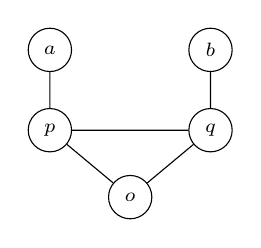
\begin{tikzpicture}[scale=0.85,every node/.style={circle,draw,inner sep=1pt,minimum size=5.5mm,font=\scriptsize}]
\node (a) at (0,1.6) {$a$}; \node (b) at (2.4,1.6) {$b$};
\node (p) at (0,0.4) {$p$}; \node (q) at (2.4,0.4) {$q$}; \node (o) at (1.2,-0.6) {$o$};
\draw (a)--(p) (b)--(q) (p)--(q) (p)--(o) (q)--(o);
\end{tikzpicture}\\{\footnotesize OR gadget $o=\mathrm{OR}(a,b)$}
\end{minipage}\hfill
\begin{minipage}{0.5\linewidth}\footnotesize
Vertices: $T,F,B$; $x_1,\overline{x_1},\dots,x_4,\overline{x_4}$; clause 1: $o_1=\mathrm{OR}(x_1,\overline{x_2})$, $o_2=\mathrm{OR}(o_1,\overline{x_3})$;
clause 2: $o_1'=\mathrm{OR}(x_1,x_3)$, $o_2'=\mathrm{OR}(o_1',x_4)$; $o_2,o_2'$ joined to $F$ and $B$. $3+8+12=23$ vertices, $3+12+24=39$ edges.\\
\textbf{Colouring} ($x_1=1$, $x_2=x_3=x_4=0$): $x_1,\overline{x_2},\overline{x_3}=T$; $\overline{x_1},x_2,x_3,x_4=F$; in every OR gadget
$p=F$, $q=B$, $o=T$ (checked: each gadget's inputs allow this). Every edge joins different colours.
\end{minipage}
\end{ans}

\begin{thm}{Theorem 11.7. Directed Hamiltonian Cycle is NP-complete.}\src{Lecture 8 pp.\,30--40}{---}\end{thm}
\begin{proof}
\emph{In NP:} certificate = the vertex order; check each vertex appears once and consecutive pairs are edges.
\emph{3-SAT $\le_p$ DIRHAMCYCLE.} For $\phi$ with $n$ variables, $m$ clauses: for each $x_i$ a \emph{row} of $3m+3$ vertices
$v_{i,1},\dots,v_{i,3m+3}$ with edges both ways between neighbours; a cycle entering a row at one end must walk straight to the other end
(turning back revisits a vertex), so each row is traversed left-to-right ($x_i=$ true) or right-to-left ($x_i=$ false). Add $s,t$: $s\to$ both
ends of row 1, both ends of row $i\to$ both ends of row $i+1$, both ends of row $n\to t$, $t\to s$. For each clause $C_j$ add a vertex $c_j$ and,
using positions $3j,3j+1$ of row $i$: if $x_i\in C_j$, edges $v_{i,3j}\to c_j\to v_{i,3j+1}$ (detour usable left-to-right); if
$\overline{x_i}\in C_j$, edges $v_{i,3j+1}\to c_j\to v_{i,3j}$ (usable right-to-left). Polynomial size.
($\Rightarrow$) For a satisfying $\alpha$, traverse row $i$ in the direction of $\alpha(x_i)$; for each $C_j$ pick a true literal and take its detour
through $c_j$ (it points the right way because the literal is true); different clauses use different positions, so detours do not interfere.
($\Leftarrow$) A detour cannot leave $c_j$ into a different row: $v_{i,3j+1}$ would then be stranded (its in-edges from $v_{i,3j}$ and $c_j$ unusable,
both of its out-neighbours already used). So each $c_j$ is a detour inside one row, whose direction makes that literal true. Read off $\alpha$ from the
row directions: every clause has a true literal.
\end{proof}

\begin{thm}{Theorem 11.8. Partition is NP-complete.}\src{Lecture 8 pp.\,47--51}{---}\end{thm}
\begin{proof}
\emph{In NP:} certificate $S$; add up both sides. \emph{Subset Sum $\le_p$ Partition.} Given $a_1..a_m$, target $t$, let $a=\sum a_i$.
\emph{Case $2t\ge a$:} add $a_{m+1}=2t-a$; the total is $2t$, so a partition has $t$ on each side. If $S\subseteq\{1..m\}$ sums to $t$, the other
side sums to $(a-t)+(2t-a)=t$: a partition. Conversely the side of a partition not containing $m+1$ is a subset of $\{1..m\}$ summing to $t$.
\emph{Case $2t<a$:} add $a_{m+1}=a-2t$; total $2a-2t$, each side $a-t$. If $S$ sums to $t$, $S\cup\{m+1\}$ sums to $a-t$. Conversely, on the side
containing $m+1$, the other elements sum to $(a-t)-(a-2t)=t$. Linear-time construction.
\end{proof}

\subsection{Space complexity}

\begin{thm}{Theorem 11.9. $\P\subseteq\PS$ and $\NP\subseteq\NPS$; overall $\P\subseteq\NP\subseteq\PS$.}\src{Lecture 9 p.\,7}{2021-22 Q13(ii); 2019-20 Q13(b)}\end{thm}
\begin{proof}
A TM that makes at most $T(n)$ moves cannot visit more than $1+T(n)$ cells (one new cell per move at most). So polynomial time implies
polynomial space, for DTMs and NTMs. Then $\NP\subseteq\NPS=\PS$ (Savitch, 11.11).
\end{proof}

\begin{thm}{Theorem 11.10. If a $p(n)$-space TM (deterministic or not) accepts $w$, $|w|=n$, it does so within $c^{1+p(n)}$ moves for a constant $c$.}
\src{Lecture 9 pp.\,8--10}{used in Savitch and in PSPACE $\subseteq$ EXPTIME (2020 Q12(b))}\end{thm}
\begin{proof}
With $s$ states and $t$ tape symbols, the number of IDs using $\le p(n)$ cells is at most $s\,p(n)\,t^{p(n)}$ (state, head position, contents).
Take $c=s+t$: $(t+s)^{1+p(n)}=t^{1+p(n)}+(1+p(n))s\,t^{p(n)}+\cdots\ge s\,p(n)\,t^{p(n)}$. A shortest accepting computation never repeats an ID
(cut out the loop otherwise), so it has fewer than $c^{1+p(n)}$ moves. Hence a counter can stop any branch after $c^{1+p(n)}$ moves without losing
acceptances --- the machine then always halts.
\end{proof}

\begin{thm}{Theorem 11.11 (Savitch). $\NPS=\PS$; more precisely $\mathrm{NSPACE}(f(n))\subseteq\mathrm{SPACE}(f^2(n))$ for $f(n)\ge n$.}
\src{Lecture 9 pp.\,11--18}{2023-24 Q12(ii); 2022-23 Q13(ii); 2021-22 Q13(iii); 2019-20 Q13(c) (TRUE)}\end{thm}
\begin{proof}
$\PS\subseteq\NPS$: a DTM is an NTM. For $\NPS\subseteq\PS$, simulate an $f(n)$-space NTM $N$ deterministically. Trying branches one by one could
need exponential space (a branch has $c^{O(f(n))}$ choices to record). Instead use
\[\textsc{reach}(I,J,m)=\text{``can $N$ go from ID $I$ to ID $J$ in at most $m$ moves?''}\]
If $m=1$: check $I=J$ or $I\vdash J$ directly. Otherwise, for every ID $K$ of size $\le f(n)$ in turn, test $\textsc{reach}(I,K,m/2)$ and then
$\textsc{reach}(K,J,m/2)$; answer yes if both hold for some $K$. The two recursive calls run one after the other, so at any time the stack holds
one frame per level: $(I,J,m),(I_2,J_2,m/2),(I_3,J_3,m/4),\dots$ --- at most $\log_2m$ frames.
To decide $w$: for each accepting ID $J$ (enumerated systematically) call $\textsc{reach}(I_0,J,m)$ with $I_0$ the initial ID and
$m=c^{1+f(n)}$ (Theorem 11.10). Then $\log_2m=O(f(n))$ frames, each holding two IDs ($1+f(n)$ cells each) and $m$ in binary ($O(f(n))$ cells):
$O(f(n))$ per frame. Total space $O(f^2(n))$ --- polynomial when $f$ is. Hence $\NPS\subseteq\PS$.
\end{proof}

\begin{ans}{Relationships and true/false (2017-18 Q13(b); 2019-20 Q13; 2020 Q12(b); 2021-22 Q13; 2023-24 Q12(i))}
Proved: $\P\subseteq\NP\subseteq\PS=\NPS\subseteq\mathrm{EXPTIME}$ (the last by 11.10: stop after $c^{1+p(n)}$ moves), and
$\P\subsetneq\mathrm{EXPTIME}$. Believed but open: $\P\ne\NP$, $\NP\ne\PS$, $\PS\ne\mathrm{EXPTIME}$.
Every NP-complete problem lies in $\NP\setminus\P$ if $\P\ne\NP$; all of these classes lie inside the recursive languages, which lie inside RE.
\begin{itemize}
\item ``SAT in P implies P = NP'' --- \textbf{True} (11.1(b), 11.2).
\item ``NP $\supseteq$ PSPACE'' (polynomial-time NTMs decide a superset of polynomial-space DTMs) --- \textbf{not known, believed false}; the
known relation is the reverse, $\NP\subseteq\PS$ (11.9).
\item ``PSPACE $=$ NPSPACE'' --- \textbf{True} (Savitch, 11.11).
\end{itemize}
\end{ans}

\end{document}
